%all_together.tex

\documentclass[11pt, a4paper, pdftex, oneside]{scrbook}

\usepackage[paper=a4paper,top=35mm,bottom =35mm]{geometry}
%\usepackage[paper=a4paper,left=35mm,right=25mm,top=35mm,bottom =40mm]{geometry}

\usepackage{float}
\usepackage{amsmath}
\usepackage{amssymb}
\usepackage{fancyhdr}
\usepackage{graphicx}
% \usepackage{subcaption}    % for subfigures
\usepackage{color}         % to be able to write text in colored ink
\usepackage[square,comma]{natbib} % to customize the citation styles...
\usepackage{multicol}      % multiple columns (needed for title page)
%\usepackage{endfloat}     % put all figures in the end, see text without them

\usepackage{array}
\usepackage[ngerman]{babel}
\usepackage{tabularx}
\usepackage{subfig}
\usepackage[utf8]{inputenc}
\usepackage{titlesec}
\setcounter{secnumdepth}{4}
\usepackage{url}

\usepackage{enumitem}
\setitemize{noitemsep,parsep=0pt,partopsep=0pt}

% internal links (when referencing a figure, section...)
% but without them making the text ugly with colored boxes
\usepackage[colorlinks=true, linkcolor=black, citecolor=black]{hyperref}

\pagestyle{fancy}
\fancyhf{}
\fancyhead[C]{\leftmark}
\fancyfoot[R]{\thepage}
% ------------------------------------------------------------------------------
% draw simple graphs directly in latex
\usepackage{tikz}
\usetikzlibrary{arrows,positioning}

% to find the figure-directory

%\graphicspath{D:\Dropbox\Bachelorarbeit\Tech\Images}
\graphicspath{{./Bilder/}}
% ------------------------------------------------------------------------------
% code input:
% \usepackage{listings}
% \lstset{escapechar=@}

% \definecolor{mygreen}{RGB}{28,172,0} % color values Red, Green, Blue
% \definecolor{mylilas}{RGB}{170,55,241}

% \lstset{language=Octave,              % kA ob das anders ist als Matlab?
%     basicstyle=\small,                % je kleiner, desto mehr zeichen pro zeile
%     breaklines=true,                  % lange zeilen umbrechen
%     keywordstyle=\color{black},        % Wörter wie "if" oder "for" in blau
%     stringstyle=\color{black},      % Strings in lila
%     commentstyle=\color{black},     % Kommentare in grün
%     captionpos=b,                     % überschrift unter das programm
%     frame=single,                     % Rahmen um code-blöcke
%     numbers=none,                     % Zeilennummern auf der linken Seite
%     numberstyle=\tiny\color{black},    % Größe und Farbe der Zeilennummerierung
% }

\hypersetup{ hidelinks, }
% ------------------------------------------------------------------------------

\begin{document}
\parindent0pt

% to have all papers in the bibliography mentioned:
% \nocite{*}
\pagenumbering{gobble}
%cover.tex

\begin{center}
	
\includegraphics[scale=0.8]{uni_os_l.png}\\

	\vspace{0.5cm}
	{\Large Fachbereich \par}
	{\Large Humanwissenschaften \par}
	{\Large Institut für Cognitive Science \par}
	\vspace{2cm}
	{\scshape\LARGE Bachelorarbeit\par}
	\vspace{0.5cm}
	{\Large Automatisierte Analyse von Preisbildungsmustern\\
	anhand von Zeitreihendaten der Markttransparenzstelle für Kraftstoffe \par}
	\vspace{2cm}
	{\LARGE Kai Fritsch \par}
	{(kai.m.fritsch@gmail.com) \par}
	\vfill
	{\LARGE \today\par}
	\vspace{2cm}
	\begin{multicols}{2}
	Erstkorrektor: \par
	{\Large Prof. Dr. Oliver Vornberger\par}
	\columnbreak
	Zweitkorrektor: \par
	{\Large Prof. Dr.-Ing. Elke Pulvermüller}
	\end{multicols}


	% \vspace*{2cm}
	% \Large
	% \textbf{Fachbereich}\\
	% \textbf{Humanwissenschaften}\\
	% \textbf{Institut für Cognitive Science}\\
	% \vspace*{2cm}
	% \Huge
	% \textbf{Bachelorarbeit}\\
	% \vspace*{0.5cm}
	% \large
	% Automatisierte Analyse von Preisbildungsmustern\\
	% anhand von Zeitreihendaten der Markttransparenzstelle für Kraftstoffe\\
	% % \vspace*{1cm}
	% % \textbf{Ausblick}\\
	% \vspace*{2cm}
	
	% \vfill
	% \normalsize
	% \newcolumntype{x}[1]{>{\raggedleft\arraybackslash\hspace{0pt}}p{#1}}
	% \begin{tabular}%{x{6cm}p{7.5cm}}
	% 	\rule{0mm}{5ex}\textbf{Autor:} & Kai Fritsch\newline kai.m.fritsch@gmail.com \\ 
	% 	\rule{0mm}{5ex}\textbf{Prüfer:} & Prof. Dr. Oliver Vornberger \\ 
	% 	% \rule{0mm}{5ex}\textbf{Abgabedatum:} & - \\ 
	% \end{tabular} 
\end{center}






% \begin{titlepage}
% 	\centering
% %	\includegraphics[width=0.5\textwidth]{uni-logo-2zeilen} \par
% 	\vspace{0.5cm}
% 	{\Large Department of Humanities \par}
% 	{\Large Institute of Cognitive Science \par}
% 	\vspace{2cm}
% 	{\scshape\LARGE Bachelor Thesis\par}
	
% 	{\Huge Automatic Graph Extraction from Biological Images \par}
% 	\vspace{2cm}
% 	{\LARGE Benjamin Uhl \par}
% 	{(buhl@uni-osnabrueck.de) \par}
% 	\vfill
% 	{\LARGE \today\par}
% 	\vspace{2cm}
% 	\begin{multicols}{2}
% 	First supervisor: \par
% 	{\Large Dr. Gordon Pipa \par}
% 	\columnbreak
% 	Second supervisor: \par
% 	{\Large Olivera Stojanovic}
% 	\end{multicols}
% \end{titlepage}


\pagenumbering{Roman}
\newgeometry{left=4.5cm,right=4cm}
\addchap*{Abstract}
\thispagestyle{empty}

Diese Bachelorarbeit beschäftigt sich mit dem Preisverhalten von Tankstellen. Es werden Preismuster in den Preisänderungen von Tankstellen gesucht, die auf regelbasiertes Verhalten zwischen einzelnen Konkurrenten hindeuten könnten. Dazu wird der Datensatz der Markttransparenzstelle für Kraftstoffe verwendet, welcher die Preisänderungen der letzten drei Jahre umfasst. Weil bereits begründete Vermutungen über die Form von derartigen Regeln bestehen, wird, anstatt der üblichen Algorithmen aus dem Bereich des maschinellen Lernens, ein auf dieses Problem zugeschnittener Algorithmus verwendet, um dieses Hintergrundwissen gewinnbringend nutzen zu können.\\ 
Die Ergebnisse zeigen, dass Regeln sicher erkannt werden können, sofern diese auch kontinuierlich angewandt werden. Zu selten umgesetzte Regeln lassen sich nicht von zufälligerweise korrelierenden Preisänderungen unterscheiden. Zudem gibt es einige sehr stark korrelierende Muster die auf Regeln hindeuten, wo jedoch nur indirekte Zusammenhänge - über die Einwirkungen dritter Tankstellen - bestehen. Zuletzt wird noch ein Ausblick auf Verbesserungsoptionen dieses ersten Ansatzes gegeben, mittels derer die Fehlerrate noch weiter gesenkt werden könnte. 
\addchap*{Danksagung}
\thispagestyle{empty}

Zuerst würde ich gerne dem kompletten zahlz-Team danken, welches mich für den Zeitraum dieser Arbeit in ihren Räumlichkeiten freundlich aufgenommen hat und auf deren Kompetenz ich jederzeit zurückgreifen konnte. Besonderer Dank gilt zum einen Sebastian Herkenhoff, der diese Arbeit überhaupt ermöglich hat und sich außerden um alle organisatorischen Angelegenheiten gekümmert hat. Zum anderen möchte ich mich besonders bei Jewgeni Kovalev - meinem Supervisor - bedanken, der mir von der Einarbeitung bis hin zum Korrektur lesen bei allen Problemen zur Seite stand.\\
Ich möchte auch der Q1 danken, die mir einige ihrer Daten als Testdaten zu Verfügung gestellt haben. Insbesondere möchte in Jonathan Burghardt danken, der sich die Zeit genommen hat, mich in die generellen Abläufe am Kraftstoffmarkt einzuweisen und mir alle meine Fragen zu beantworten.\\
Zuletzt will ich mich ganz herzlich bei meiner Mutter Ulrike und meiner Lebensgefährtin Natalie bedanken, die sich die Zeit genommen haben, mich bei Stil- und Designfragen zu beraten und die Unmengen an Tipp- und Zeichensetzungsfehlern zu entfernen.

\clearpage


\restoregeometry

\tableofcontents
\listoffigures

\clearpage
\newcounter{ro}
\setcounter{ro}{\value{page}}
\pagenumbering{arabic}
%einleitung.tex
\chapter{Einleitung}
\label{sec:Einleitung}

\section{Geschichtlicher Hintergrund}
Kraftstoffpreise unterliegen nun schon seit längerer Zeit großen Preisschwankungen. Die hohe Homogenität und sinkende Nachfrage sind optimale Bedingungen für starken Konkurrenzdruck. Der Druck ist so hoch, dass die Anzahl an Tankstellen in Deutschland seit 1970 von gut 46.000 auf heute knapp 15.000 gefallen ist \citep*{PraTa}. Trotzdem ist die Anzahl an Preisänderungen in den letzten Jahren noch einmal merklich gestiegen. Während der Preis 2011 an Tankstellen jeweils durchschnittlich weniger als zwei mal pro Tag geändert wurde, sind sie inzwischen größtenteils bei um die sechs Änderungen pro Tag angelangt \citep*{Unity}. \\

%TODO: Check for Pricings per Day for each month since start\\

Mitgrund für diese jüngste Steigerung könnten dieses Mal jedoch die neuesten elektronischen Möglichkeiten sein. Während Tankstelleninhaber vor einigen Jahren noch ihrer Konkurrenz einen Besuch abstatten mussten um deren Preise auszukundschaften, reicht heute eine Suchanfrage im Internet. Und selbst diese ist seit der Einführung der Markttransparenzstelle für Kraftstoffe nicht mehr notwendig. Jede Tankstelle ist seit Ende 2013 verpflichtet, ihre Preisänderungen dem Bundeskartellamt für Kraftstoffe elektronisch zu übermitteln. Der auf diese Weise entstandene Datensatz  bildet die Grundlage dieser Arbeit.\\

\section{Pricing Strategien}
Tankstellen waren in den letzten Jahren immer wieder gezwungen, ihre Strategien dem immer schneller werdenden Markt anzupassen. Die neu eingeführte zentrale und unmittelbare Verfügbarkeit aller aktuellen Preise ermöglicht es Tankstellenbesitzern, ihre Preise innerhalb kürzester Zeit an die Konkurrenz anzupassen. Das Bestehen einer einheitlich definierten Schnittstelle ermöglicht es auch, Preisänderungen zunächst automatisch zu registrieren und anschließend die davon betroffenen eigenen Preise anhand von Regeln ebenfalls automatisch anpassen zu lassen. Neben den offensichtlichen Vorteilen, wie zum Beispiel der Einsparung von Arbeitskräften, birgt diese Automatisierung aber auch Probleme.\\
Solange Preise noch mit viel Aufwand manuell verglichen werden mussten, war es nur möglich einen sehr kleinen Kreis an anderen Tankstellen zu überwachen um mit deren Preisen zu konkurieren. Die Vereinfachung der Arbeit durch automatische Prozesse führt dazu, dass mehr Konkurrenten bei gleichzeitig geringerem Aufwand überwacht werden können. Zudem können die gewünschten Reaktionen viel zuverlässiger durchgeführt werden. Das führt zu einem generellen Anstieg an Preissenkungen und damit auch zu einer allgemeinen Senkung der eigenen Preise. Um dem entgegen zu wirken, müssen diese zu Anfang des Tages höher angesetzt werden. Inzwischen wurde sogar eine sogenannte Mittagserhöhung eingeführt, um dem Preisverfall entgegen zu wirken. Auch eine gewisse Abstimmung von Preisen zwischen den Konkurrenten wird immer wichtiger. Wollen zwei Tankstellen jeweils einen günstigeren Preis fahren als die jeweils andere, so würde der Preis kontinuierlich sinken, bis eine Tankstelle ihr Minimum erreicht hat. Es gibt unter Tankstellen deshalb so etwas wie eine Rangordnung, die den Markt in A-Preiser und B-Preiser unterteilt. A-Preiser, zumeist die Markentankstellen, erlauben den B-Preisern, zumeist freie Tankstellen oder kleinere Tankstellenketten, etwas geringere Preise zu fahren. Während der Preisverfall bei einem Verstoß gegen diese Rangordnung vor der Automatiserung noch relativ langsam von voranging, fällt der Preis bei automatischem Pricing innerhalb weniger Minuten auf das Minimum. Zudem müssen jegliche Art von Sonderfällen in den Regeln berücksichtigt werden, da schon kleine Fehler große Verluste erzeugen könnten. Um ungewünschten Preisen durch einen vollautomatischen Betrieb vorzubeugen, beschränkt sich der automatisierte Part des Pricings teilweise auf den Vorschlag von Preisänderungen, welche dann noch manuell durchgeführt werden müssen.\\

\section{Motivation}
Die Idee dieser Arbeit besteht darin, das Konkurrenzverhalten der Tankstellen zu analysieren. Es ist anzunehmen, dass eine Tankstelle, egal ob sie ihre Preise manuell oder automatisch verwaltet, versucht diese möglichst gewinnoptimierend zu gestalten. Preise werden demnach im Allgemeinen nach bestimmten Richtlinien und in Abhängigkeit von verschiedenen Parametern festgelegt. In den Fällen, wo Entscheidungen konsistent nach bestimmten Parametern getroffen werden, entsteht im Grunde regelbasiertes Verhalten. Das unterschiedliche Verhalten erlaubt im Gegenzug Rückschlüsse auf die zu Grunde liegenden Regeln. Je konsistenter eine Regel umgesetzt wird, desto einfacher ist es, diese anhand ihrer Auswirkungen zu rekonstruieren. Je automatisierter also eine Tankstelle ihr Pricing betreibt, desto einfacher sollte es sein, ihr Verhalten zu analysieren.\\

\subsection{Unmittelbarer Nutzen}
In einem Wettbewerb ist es immer von Vorteil, die Strategien der Konkurrenten zu kennen. Es ermöglicht eine akkuratere Vorhersage des zukünftigen Marktgeschehens und hilft dabei, die eigene Strategie gewinnbringender zu gestalten. Da das Pricing in großen Tankstellenketten zentral betrieben wird, liegt die Verantwortung für das Preisverhalten von mehreren Hunderten Tanstellen bei einem sehr kleinen Personenkreis. Angenommen diese Personen würde gerne das Verhalten ihrer Konkurrenten vorhersagen können und würden versuchen die Regeln eigenhändig zu ermitteln. Bei beispielsweise 100 Tankstellen mit jeweils fünf potentiellen Konkurrenten und sechs Preisänderungen pro Tag müssten diese Personen Regeln für 500 Konkurrenten in 3000 Preisänderungen pro Tag erkennen. Eine automatisierte Regelerkennung würde also viel Arbeit und Mühen ersparen und wahrscheinlich sogar verlässlichere Ergebnisse liefern. Die eingesparte Zeit kann dann in die Optimierung des eigenen Verhaltens investiert werden, wofür die verlässlicheren Ergebnisse eine viel bessere Grundlage darstellen.\\

\subsection{Potentielle Möglichkeiten}
Jede Preissenkung verringert die Gewinnspanne einer Tankstelle. Es liegt also prinzipiell nicht im Interesse einer Tankstelle, Preise zu senken. Angenommen, eine automatisierte Regelerkennung wäre gegeben. Es bestünden dann einige Möglíchkeiten, dieses Wissen gewinnbringend zu nutzen:
\begin{itemize}
\item Mit einer solchen Regelerkennung ließen sich reaktive Preisänderungen von aktiven unterscheiden. Einzelne Änderungen könnten somit iterativ über die jeweiligen auslösenden Konkurrenten zurückverfolgt werden bis hin zu einer aktiven Änderung, also dem eigentlichen Auslöser. Die Erkennung der Initiatoren von Preissenkungen bietet die Möglichkeit auf solche Änderungen anderweitig zu reagieren und Senkungswellen zu umgehen.
\item Ebenso denkbar wäre, dass es Auslöser in Form von aktiven Senkungen gar nicht so häufig gibt wie angenommen. Einige Tankstellen reagieren zwar bei ihren Preissenkungen auf ihre Konkurrenz, legen ihre Tagesstartpreise aber unabhängig fest und führen die übrigen Erhöhungen eigenständig durch. Eine Tankstelle, die ihre Tagesstartpreise weniger hoch ansetzt, wäre somit potentieller Auslöser von einer Senkungswelle, weil andere Tankstellen mit schon bestehenden Preisen darauf reagieren müssen. Es wäre also unter Umständen möglich, dass sich einige Tankstellen, auch in eigenem Interesse, intensiver mit den eigenen Erhöhungen beschäftigen müssten.
\item Es ist bereits ohne dieses Tool möglich, einige Preisänderungen grob über größere Strecken zurückzuverfolgen. Mit dem Tool bestünde die Möglichkeit, die genauen Verkettungen von Konkurrenten zu erkennen und so Preiswege exakt darzustellen. Man könnte dann versuchen, diese Ketten zu unterbrechen, sodass isoliertere Preissektoren entstünden und Senkenswellen kleinere Umfänge hätten.
\item Die Auswertung der Ergebnisse bezüglich der eigenen Tankstellen bietet auch die Möglichkeit, die eigenen Änderungen systematisch zu analysieren und und weniger wichtige Konkurrenten aus dem System zu nehmen.
\end{itemize}
Diese Änderungen müssen jedoch nicht zwangsläufig nur den Tankstellen zugutekommen. Eine Tankstelle ist gesetzlich verpflichtet, keine verlustbringenden Preise zu fahren, um Preisdumping zu vermeiden. Sie muss somit die ganzen Preissenkungen an einem Tag in die Preiserhöhung zu Tagesbeginn einkalkulieren. Das ist höchstwahrscheinlich auch ein Grund für die erst kürzlich eingeführte Mittagserhöhung. Eine Verminderung der Preissenkungen führt somit nicht zwangsweise zu höheren Preisen, da der Wettbewerb weiterhin besteht. Sie sollte vielmehr zu generell stabileren Preisen führen, sodass Kunden sich besser auf Preise einstellen können.
%grundlagen.tex
\chapter{Grundlagen}
\label{sec:Grundlagen}

Dieses Kapitel soll einen Überblick über die für diese Arbeit zur Verfügung stehenden Informationen sowie die darin verwendeten Tools verschaffen. Zu den Informationsquellen zählen zum einen der Datensatz der Markttransparenzstelle(MTS) für Kraftstoffe, sowie zum anderen der exemplarische Aufbau eines der auf dem Markt verfügbaren automatischen Pricing-Tools. Zusätzlich dazu liegt auch ein Erfahrungsbericht vor, wie dieses Tool bei einer Tankstelle eingesetzt wird.

\section{Datensatz}
\begin{quote} 
\glqq Seit dem 31. August 2013 sind Unternehmen, die öffentliche Tankstellen betreiben oder über die Preissetzungshoheit an diesen verfügen, verpflichtet, Preisänderungen bei den gängigen Kraftstoffsorten Super E5, Super E10 und Diesel in Echtzeit an die Markttransparenzstelle für Kraftstoffe zu melden \citep*{BkMTS}.\grqq
\end{quote}

In Echtzeit bedeutet, dass die Information über eine Preisänderung spätestens 5 Minuten nach der Änderung selber an der MTS eingehen muss. Neben den Preisänderungen müssen auch die Stammdaten der Tankstellen wöchentlich an die MTS gemeldet werden. Die MTS veröffentlicht die Daten nicht direkt selber, sondern stellt sie Verbraucherinformationsdiensten(VID) zur Verfügung. Diese verpflichten sich, die Daten in einer den Verbrauchern nützlichen Form zu veröffentlichen. Die Schnittstelle der MTS ist in der \autoref{fig:MTSK} dargestellt \citep*{IMTSK}.

\begin{figure}
	\center
	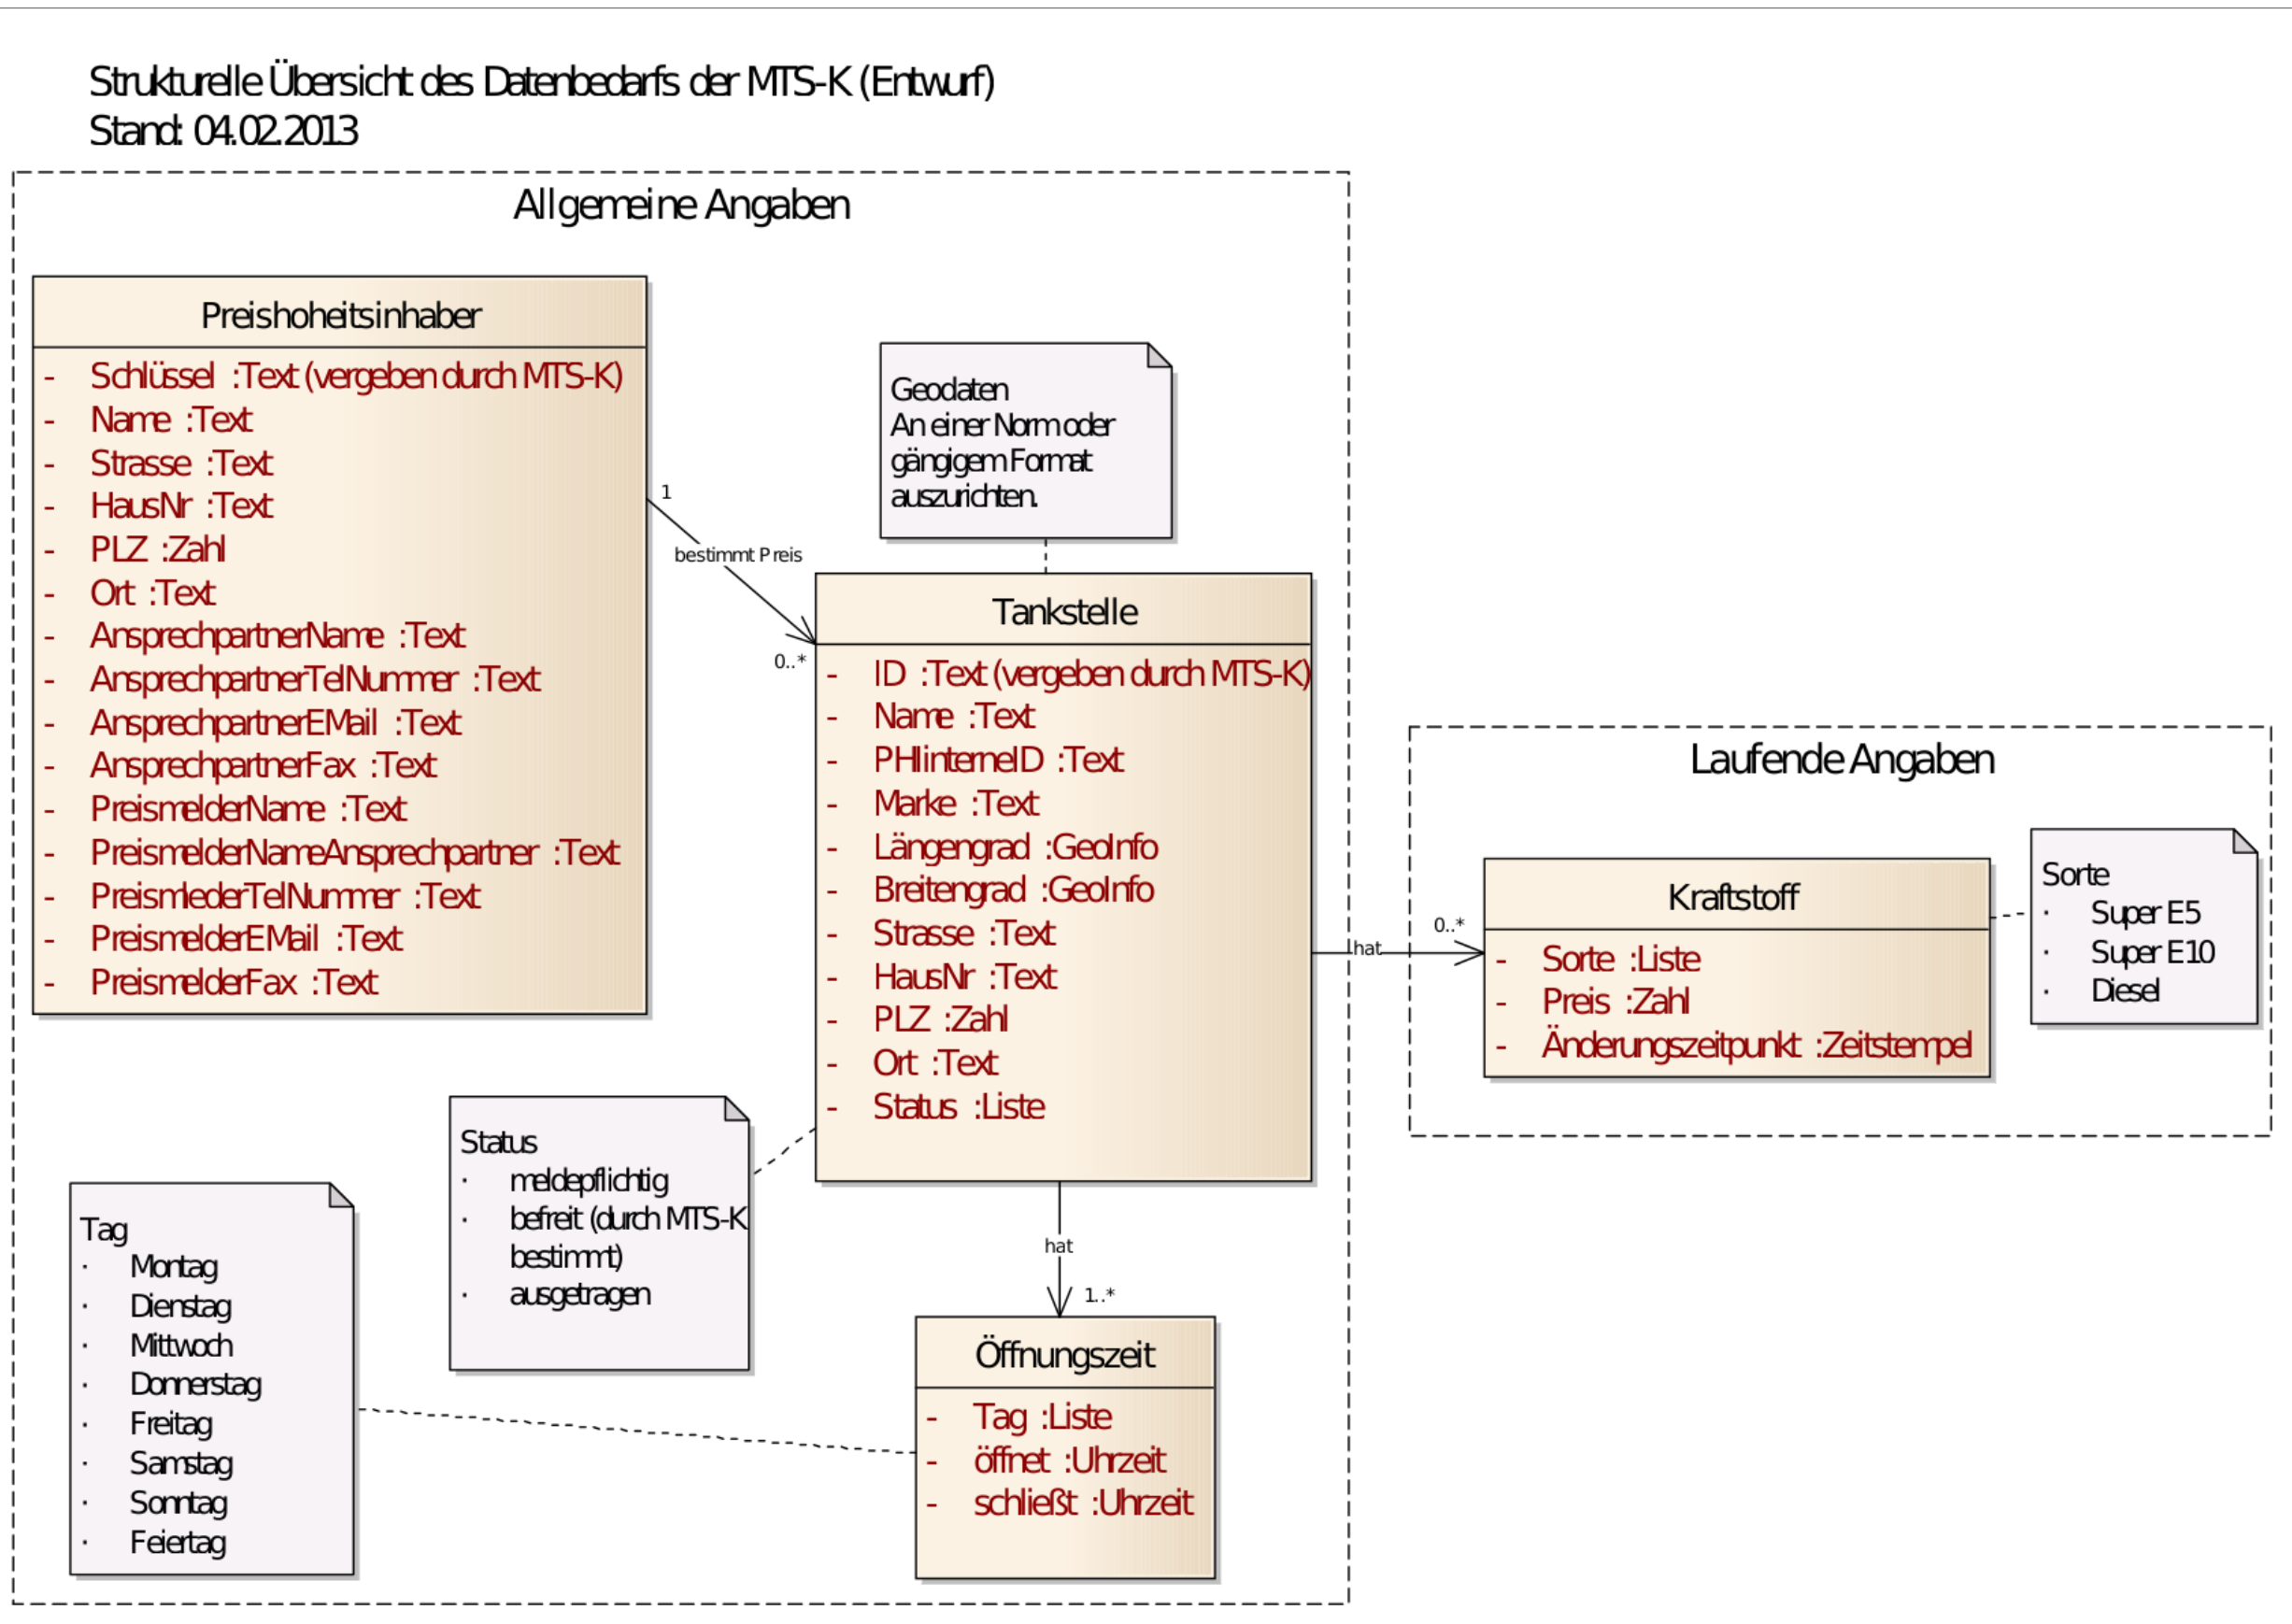
\includegraphics[width=0.8\textwidth]{Bilder/Datenstruktur-MTS.png}\\
	\caption{Datenstruktur der MTS für Kraftstoffe}
	\label{fig:MTSK}
\end{figure}

Der Datensatz für diese Arbeit entstammt dem Verbraucherinformationsdienst der \glqq Tankerkönig API \grqq. Tankerkönig bezieht seine Daten direkt von der MTS  und stellt diese sowohl im Zuge einer Echtzeit-Benzinpreis-API als auch gesondert aufbereitet als historische Datenbank in Form eines PostgreSQL-Dumps im 9.4.-Format zur Verfügung. Die für diese Arbeit verwendeten Dumps umfassen neben den kompletten Preisdaten vom 8.6.2014 bis zur aktuellsten Änderung auch die Informationen über die Stammdaten der Tankstellen \citep*{TkAPI}. 

\begin{figure}
	\center
	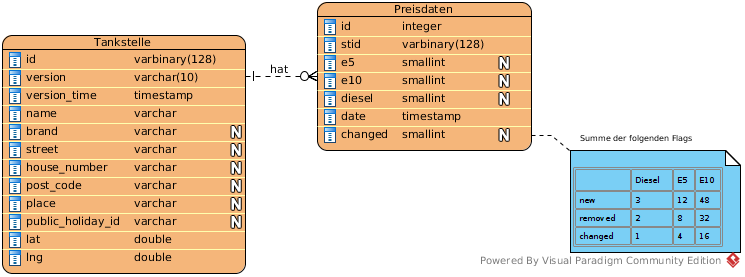
\includegraphics[width=0.8\textwidth]{Bilder/pricing_data.png}\\
	\caption{Entity-Relationship-Diagram des historischen Datensatzes}
	\label{fig:ERDT}
\end{figure}

Alle für diese Arbeit verfügbaren Informationen sind in der \autoref{fig:ERDT} abgebildet. Die Daten aus dem MTS-Datensatz werden größtenteils von den Tankstellen selber zur Verfügung gestellt, weshalb die Datenfelder teilweise nicht einheitlich definiert sind. Nur der Identifikator einer Tankstelle wird von der MTS selber bereitgestellt. Die Felder \textit{$version\_timestamp$} und \textit{version} wurden dem Datensatz von Tankerkönig hinzugefügt und geben Auskunft darüber, wann Änderungen an den Stammdaten einer Tankstelle vorgenommen wurden, beziehungsweise zählen die verschiedenen Versionen. Die Felder \textit{name} und \textit{brand} werden von den Tankstellen selber befüllt und enthalten sehr verschiedene Informationen. Bei großen Markentankstellen wird unter \textit{brand} die Marke geführt und als \textit{name} wird oft die Adresse der jeweiligen Tankstelle aufgeführt, da diese offenbar zur Identifizierung innerhalb des Unternehmens genutzt wird. Einzelne Tankstellen oder kleinere Unternehmen führen hingegen unter \textit{brand} entweder überhaupt keine Angaben oder verschiedene Bezeichnungen dafür, dass diese Tankstellen keinem größeren Konzern angehören. Bei \textit{name} geben Sie dann meistens den Inhaber oder den Unternehmensnamen an. Bei den Datenfeldern zur Adresse fehlen teilweise Informationen oder es werden Felder zusammengenommen. Beispielsweise taucht die Hausnummer des öfteren bereits im Straßenfeld mit auf. Um den Standort einer Tankstelle trotzdem eindeutig identifizieren zu können wird zusätzlich die Geolocation als Latitude and Longitude zur Verfügung gestellt. Die \textit{publi\_holiday\_id} gibt an, welchem Bundesland dieser Standort angehört um damit die entsprechend geltenden Feier- und Ferientage bestimmen zu können.\\
Bei den Preisänderungen hat Tankerkönig die neu angeschlagenen Preise der Kraftstoffsorten Diesel, E5 und E10, den Identifier der Tankstelle \textit{stid}, und den Zeitstempel \textit{date} übernommen. Zudem wurde unter \textit{id} ein Zähler über alle Änderungen, sowie mit \textit{changed} ein Kennwert für die geänderten Kraftstoffsorten hinzugefügt. Dieser Kennwert errechnet sich aus der Summe der jeweiligen Felder der kleinen Tabelle und gibt nicht nur an, ob ein Preis geändert wurde, sondern auch, ob dieser auf null gesetzt (removed), oder von Null kommend wieder erhöht (new) wurde.\\

\section{Pricing-Tool}

Neben den Verbrauchern können natürlich auch die Tankstellenbesitzer auf diese Daten zurückgreifen. Die einheitlich definierte technische Informationsschnittstelle ermöglicht es, Preise automatisch ohne Zeitverzögerung anzupassen. Zudem sind Kraftstoffe sehr homogene Güter. Homogen bedeutet, dass der Kunde das Produkt rein nach dem Preis auswählt, weil dieses an sich zwischen den Anbietern keine nennenswerten Unterschiede aufweißt. Das sorgt dafür, dass die Regeln nach denen Preise gestaltet werden eine dementsprechend einfache Struktur aufweisen können. Aus diesem Grund sind in den letzten Jahren einige Pricing-Tools enstanden, die die Preisgestaltung zumindest teilweise automatisieren. Während mittelständische Unternehmen auf externe Software Lösungen zurückgreifen, so wie zum Beispiel die Q1 und Westfalen AG auf Angebote der Firmen Temiz4u\footnotemark[1] und Weat\footnotemark[2], ist anzunehmen, dass zumindest die größten fünf Mineralölkonzerne Deutschlands (Aral, Shell, Jet, Esso und Total) intern entwickelte Programme verwenden dürften. Im Folgenden werden am Beispiel eines Tools die Einstellungsmöglichkeiten für den  Nutzer erklärt, die diesem bei der Definition seiner Regeln zur Verfügung stehen. Diese Optionen stellen gleichsam die Parameter dar, die im Zuge dieser Arbeit aus dem Datensatz extrahiert werden sollen.

\footnotetext[1]{Quelle: \url{https://www.temiz4u.net/web/guest/solutions}}
\footnotetext[2]{Quelle: \url{http://www.weat.de/produkte/pricing/}}

\subsection{Funktionsweise}
Im Folgenden werden die für diese Arbeit relevanten Funktionen eines solchen Tools beschrieben. Es wird für diese Arbeit angenommen, dass andere Tools inhaltlich ähnlich funktionieren. Das hier vorgestellte Tool erhält über einen oder mehrere Verbraucherinformationsdienste die aktuellen Preisänderungen aller Tankstellen. Beim Eintreffen einer Änderung wird überprüft, ob diese Änderung eine von dem Nutzer hinterlegte Regel verletzt. Wird eine Regel verletzt, wird darauf in der wiederum vom Nutzer gewählten Art und Weise reagiert. Die Nutzereinstellungen lassen sich in die drei Teilaspekte, \textit{Konkurrenten bestimmen, Regel festlegen und Automatisierungsgrad wählen} gliedern. 

\subsection{Konkurrenz bestimmen}
\begin{figure}[!ht]
	\center
	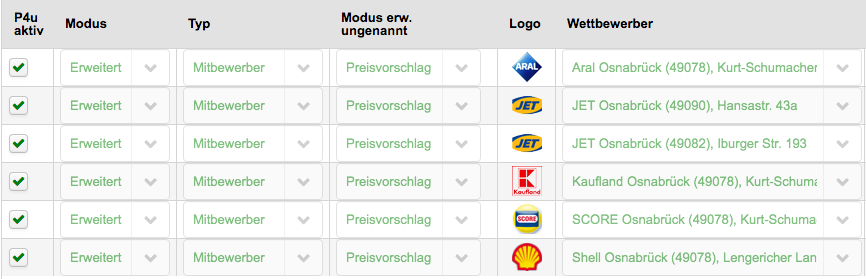
\includegraphics[width=0.8\textwidth]{Bilder/konkurenz.png}\\
	\caption{Princing Tool Einstellungsoption - Konkurrenz}
	\label{fig:PTK}
\end{figure}
Hier wird eine Liste von Tankstellen zusammengestellt, die als Konkurrenten erachtet werden. Diese Liste dient als erster Filter für die einkommenden Änderungen. Es werden im weiteren nur Änderungen überprüft, deren Tankstelle in dieser Liste vorzufinden ist.

\subsection{Regeln festlegen}
\begin{figure}[!ht]
	\center
	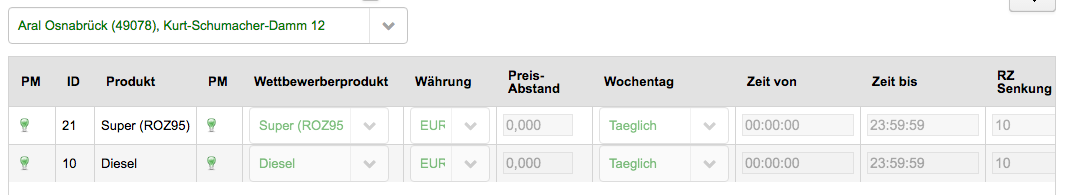
\includegraphics[width=0.8\textwidth]{Bilder/regeln1.png}\\
	\caption{Princing Tool Einstellungsoption - Regeln}
	\label{fig:PTR}
\end{figure}
Für jeden Konkurenten kann ein eigenes Regelwerk angelegt werden. Jede Regel legt zunächst einen untersten Preisabstand für eine bestimmte Spritsorte fest, welcher zu dem jeweiligen Konkurrenten gewahrt werden soll. Positive Werte besagen, dass die Tankstelle selber maximal um den genannten Betrag teuerer sein will als der entsprechende Konkurrent. Negative Werte besagen, dass die Tanstelle selber mindestens um diesen Betrag günstiger sein möchte als ihr Konkurrent. Bei dem Beispiel im Bild wären also gleiche und günstigere eigene Preise erlaubt. Zusätzlich können für den gewählten Abstand die Wochentage sowie die jeweilige Uhrzeit gewählt werden, während derer der Abstand einzuhalten ist. Wird der Abstand außerhalb dieses Zeitintervalls unterschritten, hat dies keine Konsequenzen. Im letzten Feld kann eine Reaktionszeit in Minuten angegeben werden. Diese besagt, wieviele Minuten nach dem Eingang einer regelwidrigen Änderung die gewählte Reaktion erfolgen soll.

\subsection{Automatisierung wählen}
\begin{figure}[!ht]
	\center
	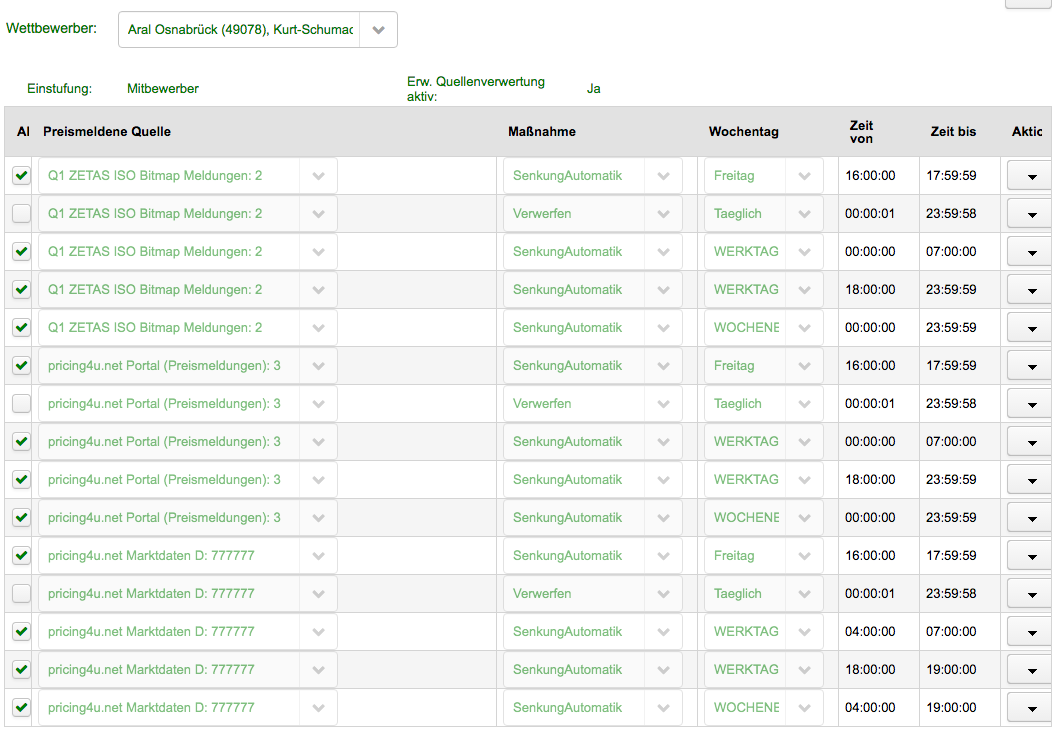
\includegraphics[width=0.8\textwidth]{Bilder/automatik.png}\\
	\caption{Princing Tool Einstellungsoption - Automatik}
	\label{fig:PTA}
\end{figure}                                                                          
Das Tool bietet neben einer \textit{default} Variante die beiden weiteren Möglichkeiten \textit{SenkungAutomatik} und \textit{Verwerfen} an, welche auf unterschiedliche Weise auf Regelverletzungen reagieren. Bei der default Variante wird bei einer Regelverletzung nach der festgelegten Reaktionszeit eine eigene Preisänderung vorgeschlagen, die den niedrigsten tolerierten Preisabstand wieder herstellt. Der Vorschlag kann dann vom Nutzer nach eigenem Ermessen durchgeführt, abgeändert oder gänzlich verworfen werden. Bei der automatischen Senkung wird anstatt eines Vorschlages die entsprechende eigene Preisänderung nach der festgelegten Reaktionszeit automatisch durchgeführt. Die letzte Möglichkeit verwirft die entsprechende Änderung ohne den Nutzer darüber zu informieren.  Wie auch schon bei den Regeln kann hier für jeden Wochentag für jedes beliebige Zeitintervall eingestellt werden, wie auf einen Verstoß reagiert werden soll.


\section{Verwendete Programme und Packages}
Das Programm zur Mustererkennung ist komplett in Python geschrieben. Es werden mit der scipy library und deren Core-Packages numpy und matplotlib die üblichen Module für den Bereich Data Mining und Machine Learning verwendet. Da die Daten als PostgreSQL-Dump zur Verfügung gestellt werden, werden sie für diese Arbeit auch wieder darin aufbereitet. Bis auf einige wenige Indexings wird von der Datenbank keinerlei Funktionalität übernommen. Indexings der Preisänderungen nach den jeweiligen Tankstellen-Ids sowie deren Zeitstempeln und der Kombination aus beiden bringt erhebliche Laufzeitverbesserungen, da die Daten hauptsächlich nach diesen Kriterien abgerufen werden. Die benötigten Daten werden mit dem PostgreSQL-Adapter psycopg aus der Datenbank geholt und dann für den kompletten Programmdurchlauf python-intern verwaltet und abgerufen. Zudem wird das Package geopy für die Berechnung des räumlichen Abstandes zwischen zwei Tankstellen anhand deren Geolocations verwendet. Die in dieser Arbeit verwendeten Visualisierungen von Barcharts, Histogrammen und anderen 2D-Graphen wurden mittels matplotlib erzeugt. Weil sich Tabellen mit diesem Tool nicht so leicht übersichtlich darstellen lassen, wurde dafür das Modul HTML.py verwendet. 
%anforderungsanalyse.tex
\chapter{Anforderungsanalyse}
\label{sec:Anforderungsanalyse}

Thema dieses Abschnittes ist es, das Ziel der Arbeit genau zu spezifizieren und zu modularisieren. Das heißt, das Ziel soll bereits in logische Untereinheiten unterteilt werden. Dafür müssen bereits absehbare Probleme erkannt und notwendige Zwischenergebnisse definiert werden.

\section{Zielsetzung}
Ziel ist es, in den Pricingdaten Verhaltensmuster zu erkennen. Es soll in dieser Arbeit ausschließlich um das Erkennen von reaktivem Verhalten gehen. Das heißt, es geht darum zu erkennen, nach welchen anderen Tankstellen sich eine Tankstelle in welchem Maße richtet. Dabei dient das Konzept des vorgestellten Tools als eine generelle Verhaltensrichtlinie. Es ist anzunehmen, dass Tankstellen, die nicht speziell dieses Tool verwenden, entweder ein sehr ähnlich gestaltetes Tool betreiben oder aber manuell nach ähnlichen Prinzipien operieren.\\
Das liegt an den Grundlagen des Wettbewerbes. Für eine Tankstelle geht es darum, einen möglichst hohen Umsatz an Kraftstofflitern zu einem möglichst hohen Preis zu erzielen. Die für den Kunden interessanten Faktoren sind hierbei in erster Linie der Preis und die Entfernung zur Tankstelle. Die Gewichtung dieser Faktoren kann sich zwischen verschiedenen Kunden und zu verschiedenen Zeiten unterscheiden. Das generelle Kundenaufkommen ist abhängig vom Verkehrsfluss, unterscheidet sich also täglich wie stündlich und teilweise auch saisonbedingt. Es sollte also im Interesse einer Tankstelle liegen, zu den für potentielle Kunden interessanten anderen Tankstellen einen konkurrenzfähigen Preisabstand zu wahren, der unter Umständen zeitlich variieren kann. Demnach sind die Parameter, nach denen in dieser Arbeit gesucht werden soll, die jeweiligen Konkurrenten einer Tankstelle, die zu diesen Konkurrenten gewahrten Preisabstände sowie der jeweilige Gültigkeitszeitraum eines Abstandes.\\
Ein weiterer Grund, sich an den Regeln der Tools zu orientieren besteht darin, dass an tatsächlich in den Tools verwendeten Regeln die Performance des verwendeten Ansatzes überprüft werden kann. Das bedeutet nicht, dass das Ziel dieses ersten Ansatzes bereits sein soll, die verfügbaren Regelsätze zu hundert Prozent nachzubilden. Es geht immer noch primär darum, die aus dem tatsächlichen Verhalten ersichtlichen Reaktionsmuster zu erkennen. Dass dies ein Unterschied ist, wird im weiteren Verlauf deutlich werden. Die Regeln sollen zunächst nur dabei helfen, die errechneten Ergebnisse auch überprüfen zu können.

\section{Generelle Voranalyse}
Im Bereich der Mustererkennung gibt es einige kritische Faktoren, welche besonders ausschlaggebend sind für das prinzipielle Vorgehen. Zunächst muss die Menge der Daten evaluiert werden. Während bei großen Datenmengen die Geschwindigkeit und der verbrauchte Speicher zu kritischen Faktoren werden, sinkt bei geringen Datenmengen schnell die Aussagekraft. Zudem haben Anzahl, Abgrenzung und Konsistenz der Muster einen großen Einfluss auf die benötigte Datenmenge. Es muss auch geklärt werden, welche Daten in welcher Form benötigt werden und wie mit fehlenden und fehlerhaften Werten umgegangen werden soll. Zuletzt müssen anhand der Auswertung der genannten Faktoren, der Art des Problems und der Verfügbarkeit von Trainingsdaten mögliche Lösungsansätze ermittelt werden.

\subsection{Datenmenge}
Der Datensatz besteht aus knapp 15000 Tankstellen und insgesammt gut 80 Millionen Preismeldungen, erfordert also aufgrund seiner Größe eine Vorstrukturierung. Eine erste Selektion der Daten ist allein durch die Struktur der gesuchten Muster bereits gegeben. Es werden preisliche Korrelationen zwischen jeweils zwei Tankstellen vermutet, was die Menge durchschnittlich auf  circa 5000 Preisänderungen pro Tankstelle reduziert. Hinzu kommt, dass die zu einer konkurrierenden Tankstelle gewählten Regeln nicht über Jahre hinweg bestehen bleiben müssen. In Anlehnung an die Funktionen des Pricing Tools wäre es möglich, dass Regeln nach einiger Zeit wechseln, nur für bestimmte Tage definiert sind oder nur für bestimmte Uhrzeiten.\\
Einmal angenommen, eine Tankstelle würde für ein halbes Jahr lang eine Regel nicht ändern, welche für drei Stunden an einem bestimmten Wochentag gültig ist. Dann würden durchschnittlich lediglich knapp 24 Änderungen in den relvanten Zeitraum fallen. Angenommen alle diese Änderungen seien  Preissenkungen und die Tankstelle hätte vier gleichwertige Konkurrenten. Dann wären es nurnoch sechs Preisänderungen, die dieser Regel entsprechen würden. Abgesehen davon, dass die Tankstelle auch noch die Möglichkeit hat, die eigenen Regeln zu ignorieren, wären das viel zu wenig Daten, um eine statistisch signifikante Aussage treffen zu können. Es muss schließlich auch noch berücksichtigt werden, dass auch genau diese sechs Änderungen als Reaktionen auf diesen Konkurrenten erkannt werden müssen.\\
Die hohe Flexibilität bei der Wahl des Zeitraumes für einen Preisabstand und die Möglichkeit Regeln nach belieben wieder zu ändern, machen es notwendig, ein paar Einschränkungen zugunsten signifikanterer Ergebnisse vorzunehmen.

\subsection{Strukturierung des Datensatzes}
Da die Datenanalyse in Python durchgeführt werden soll müssen die Daten also zunächst von der Datenbank importiert werden. Aufgrund der Menge der Daten sollten nur diejenigen importiert werden, die für die Analyse einer Tanstelle benötigt werden. Die Daten sollten so in Python abgespeichert werden, dass besonders einfach und schnell auf die benötigten Datensätze zugegriffen werden kann. Dazu muss herausgearbeitet werden, nach welchen Kriterien besonders häufig auf Daten zugegriffen wird. Es muss auch untersucht werden, ob zusätzliche Daten benötigt werden oder Datenfelder unnötig sind. Auch die jeweiligen Datentypen  der einzelnen Felder müssen eventuell geändert werden.\\
Da die Daten zu einer Preisänderung von den Tankstellen selber angegeben werden, weisen sie ein paar strukturelle Unterschiede auf, welche berücksichtigt werden müssen. Zunächst ist es möglich, pro Kraftstoffsorte eine eigene Preisänderung vorzunehmen, oder aber die Änderungen in Gruppen durchzuführen. Dann gibt es Tankstellen, die vor jeder Änderung den Preis zunächst erst einmal auf Null setzen, bevor sie ihn wieder auf den eigentlich gewünschten Stand anheben. Auch senken einige Tankstellen den Preis bei Tagesende auf Null herab. In einigen Fällen werden Preise für die selbe Kraftstoffsorte in kürzester Zeit mehrmals geändert. Alle diese Vorgehensweisen haben potentiell verschiedene Auswirkungen auf eine automatische Analyse. Es muss einerseits überprüft werden, ob die strukturellen Unterschiede unwichtig sind und im Vorhinein angeglichen werden können oder aber wichtige Informationen enthalten und deshalb bewahrt werden sollten. Dabei muss der ganze Verlauf des Programmes berücksichtigt werden, um Probleme im späteren Verlauf zu vermeiden. Das selbe gilt auch im Bezug auf den Umgang mit fehlerhafte, fehlende oder wenig sinnvolle Daten.\\

\subsection{Algorithmen und andere Ansätze}
Zunächst geht es bei dem Problem darum zu entscheiden, ob eine bestimme Tankstelle auf eine Andere reagiert oder nicht. Das macht es unter anderem auch zu einem bivalenten Klassifizierungsproblem. Eine Konkurrenz lässt sich anhand der Existenz von regelmäßigem reaktivem Verhalten erkennen. Der einfachste Ansatz bestünde darin ein Set aus möglichen Regeln zu erstellen und diese alle anhand der Daten auf ihre Gültigkeit zu untersuchen. Das ist jedoch nicht möglich, weil die Anzahl an möglichen Regeln durch den variablen zeitlichen Parameter viel zu groß ist. Die wirklichen Regeln müssen also in den Daten erkannt werden. Es müssten also zunächst diejenigen Preisänderungen bestimmt werden, die zu einer Regel gehören. Da die Regeln selber noch nicht bekannt sind, können zunächst einmal nur die Preisänderung  bestimmt werden, die potentiell die Reaktion auf eine andere Preisänderung darstellen. Es müsste nach Paarungen von potentiell auslösenden Preisänderungen und den dazugehörigen Reaktionen in den kompletten Datensätzen zweier Tankstellen gesucht werden. Dazu muss jedoch zunächst bestimmt werden, wie so eine Paarung definiert ist.\\

Eine Möglichkeit, Reaktionen zu definieren und anschließend zu klassifizieren wäre es, Methoden aus dem Bereich des maschinellen Lernens zu verwenden. Diese Methoden benötigen zur Definition eines Modells, anhand dessen über einzelne Paarungen entschieden werden kann, klassifizierte Trainingsdaten, das heißt Paarungen bei denen bekannt ist, ob diese Reaktionen sind oder nicht. Als Trainingsdaten stehen jedoch nur wenige exemplarische Regeln eines einzigen Tankstellenunternehmens zur Verfügung. Man könnte mittels dieser Regeln versuchen einige Reaktionen aus dem Datensatz zu extrahieren. Das Ergebnis wäre jedoch kein repräsentativer Auszug aus dem Datensatz, da einerseits zu wenige Regelsätze zur Verfügung stehen und andererseits nur das Verhalten eines einzigen Anbieters enthalten ist. Das Modell würde also selbst wenn die Menge der Trainingsdaten ausreichend wäre nur die Charakteristiken einer Tankstelle lernen und wäre damit nicht auf die anderen Tankstellen übertragbar.\\

Alternativ käme in Frage die Reaktionen als kausale Ereignisse zu betrachten und die aus den Zeitstempeln erstellbaren Zeitreihen mittels statistischer Methoden auf Korrelationen zu untersuchen. Zur Analyse von Kausalität in Zeitreihendaten werden oftmals verschiedene Variationen des Granger Causality Tests verwendet. Bei diesem Test wird generell geprüft, ob Ereignisse aus zwei Zeitreihen in kausaler Relation stehen. Zeitreihe A wäre nach diesem Test kausal abhängig von Zeitreihe B, wenn die Vorhersage des jeweils nächsten Ereignisses in Zeitreihe A signifikant verbessert werden würde, wenn man als Parameter neben den vorherigen Werten von A auch die vorherigen Werte aus der Zeitreihe B hinzunimmt. Für einen solchen Test müssten zunächst Zeitreihen aus den Preisänderungen generiert werden. Da Reaktionen innerhalb von kürzester Zeit erfolgen können, müssten geringe Zeitintervalle gewählt werden. Das würde zu Zeitreihen mit fast ausschließlich gleichen Werten führen, weil der Preis oft über mehrere Stunden hinweg gleich bleibt. Ein Vorhersagemodell, das immer den gleichen Preis vorhersagt, wäre also nicht mehr signifikant zu übertreffen, weil es bereits eine Trefferquote von annähern 100\% besäße. Man könnte versuchen, dieses Problem zu umgehen und die Zeitintervalle, in denen keine Änderungen stattfindet, ausschneiden. Selbst wenn eine Konkurrenz besteht sind aber nicht alle Preisänderungen Reaktionen auf nur eine Tankstelle. Man müsste also die oben beschriebene Selektion von potentiellen Reaktionspaarungen trotzdem durchführen. Selbst dann bestünde noch das Problem, dass mehrere verschiedene Regeln für die Reaktionen verantwortlich sind. Der Algorithmus prüft jedoch nur, ob Zeitreihen generell korrelieren. Man müsste die Reaktionen also nochmals nach den möglichen Abstandswerten für Regeln unterteilen. \\

Bei dieser Vielzahl an Faktoren, nach denen die Daten vorselektiert werden müssen, machen die meisten allgemein verwendeten Algorithmen wenig Sinn. Da es ohnehin notwendig ist die Daten auf die Problemstellung zugeschnittene vorzusortierung, ist es auch denkbar die Regeln mittels einfacher statistischer Mittel aus den Datengruppierungen zu ermitteln. Die Regeln sind inhaltlich über einen Preisabstand definiert. Es sind also nicht absolute Preise, sondern die Differenzen zu den Konkurrenten, die wirklich entscheidend sind. Es müsste also eine detailliert Analyse über diese Differenzen durchgeführt werden. Auch ist nicht jeder Differenzwert gleich interessant. Besonders wichtig sind nur die vergleichsweise hohen Preisabstände. Die Differenz wird aus dem Blickwinkel der reagierenden Tankstelle errechnet, wobei negative Werte bedeuten, dass diese Tankstelle einen niedrigeren Preis aufweist als der jeweilig betrachtete Konkurrent. Hohe Differenzen bedeuten für die reagierenden Tankstellen einen verhältnismäßig ungünstigen Preisabstand, wenn mit ungünstig hier die Attraktivität für Kunden gemeint ist. Der in der Regel festgelegte Preisabstand bildet also einen maximalen Schwellenwert, der nicht überschritten werden darf. Die maximalen Differenzen bedeuten also, sofern sie keine Ausreißer darstellen, den Schwellenwert der Regel. Solche logischen Überlegungen sind möglich, weil die Struktur der gesuchten Regeln bereits bekannt ist, können aber bestenfalls nur schwer in allgemeine Algorithmen eingebunden werden. Aufgrund dieser Überlegungen wird in diesem Ansatz eine problemspezifische Lösung erstellt.

\section{Modularisierung}
Aufgrund der großen Datenmenge sollten die Tankstellen einzeln analysiert werden, anstatt alle in einem Durchlauf abzuarbeiten. Auch wenn es eventuell möglich wäre, auch die Konkurrenten einer Tanstelle einzeln zu analysieren, ist es unter Umständen hilfreich, alle potentiellen Konkurrenten gleichzeitig zu untersuchen. Da nur jeweils eine Preisänderung pro eigenem Pricing als tatsächlicher Auslöser in Frage kommt, könnten so verschiedene potentielle Auslöser verglichen werden.
% Aus diesem Grund wird die Analyse einer Tankstelle auch nicht direkt zweiseitig durchgeführt. Damit wäre gemeint, für eine Tankstelle sowohl die Reaktionen auslösenden Tankstellen, als auch die auf diese Tankstelle reagierenden Tankstellen zu ermitteln. In Verbindung mit dem Ansatz alle potentiellen Konkurrenten gleichzeitig zu untersuchen würde eine zweiseitige Betrachtung zu größeren Verkettungen führen, da bei der Analyse der reagierenden Tankstellen auch wieder deren komplettes Set an möglichen Auslösern verglichen werden müsste. Deshalb werden nur die Reaktionen auslösenden Konkurrenten eines Standortes bestimmt.
Zudem kann ein Zeitraum angegeben werden, für den die Analyse einer Tanstelle durchgeführt werden soll.\\
Um nicht alle anderen 15000 Tankstellen anhand ihres tatsächlichen Verhaltens überprüfen zu müssen, sollte eine erste Vorauswahl getroffen werden. Alle wirklichen Konkurrenten auszuwählen hat dabei höhere Priorität als die Auswahl gering zu halten. Anschließend müssen für jede Preissenkung der untersuchten Tankstelle die möglichen Auslöser in den potentiellen Konkurrenten gesucht werden. Zudem werden bei jedem potentiellen Konkurrenten die Preisänderungen ermittelt, auf die nicht reagiert und mit den zu diesem Zeitpunkt gelten Preisen der untersuchten Tankstelle gepaart. Für die Summe aller Preispaarungen für den jeweiligen Konkurrent wird dann die Verteilung der Preisdifferenzen erstellt. Von den Maximalwerten abwärts wird dann auf mögliche Regeln überprüft.
%umsetzung.tex
\chapter{Umsetzung}
\label{sec:Umsetzung}

\section{Datenaufbereitung}
Mit Hilfe des Python Modules \textit{psycopg2} werden die benötigten Daten aus der Datenbank nach Python importiert. 

\subsection{Tankstellendaten}
Der komplette Datensatz an Stammdaten zu den einzelnen Tankstellen wird als Instanzen der Klasse \textit{station} in einem \textit{dictionary} abgelegt, sodass jede Tankstelle über ihre \textit{id} abgerufen werden kann. Jedes einzelne Feld wird entweder übernommen oder - falls nicht verfügbar - mit einem Defaultwert gekennzeichnet. Der Großteil der benötigten Funktionalitäten wird über diese Klasse \textit{station} bereitgestellt.  

\subsection{Preisdaten}
Die für die Analyse benötigten Preisdaten einer Tankstelle werden in einer Matrix chronologisch gespeichert. Bis auf die Tanstellen-Id werden alle Felder übernommen. Der Zeitstempel wird in Zahlenwerte für das Datum und die Uhrzeit umgerechnet. Das Datum besteht in dem Abstand zum Datum der ersten Änderung in Tagen und die Uhrzeit in den an dem Tag vergangenen Sekunden. Aus dem Datum wird zusätzlich der Wochentag bestimmt und als Zahlenwert abgespeichert. Zu den jeweiligen aktuellen Preisen werden auch die Änderungsbeträge für jede Kraftstoffsorte ermittelt. Jede Form der Preisänderung wird bis auf einen Ausnahmefall so erhalten, wie sie ist. Die Struktur ist von Bedeutung, wenn es darum geht, inhaltlich zu bestimmen, welche Änderungen potentiell ein Auslöser sein könnten. Die Ausnahme ist, wenn Preise auf Null herabgesenkt werden. Diese Fälle würden extreme Differenzwerte erzeugen, welche in der Ermittelung der Schwellenwerte für die Regeln Fehler erzeugen könnten. Außerdem stellen sie inhaltlich keine wirkliche Preisänderung dar. In diesen Fällen wird für die entsprechende Kraftstoffsorte der bis dahin geltende Preis genommen. Würde durch diese Abwandlung ein Pricing entstehen, das keine Änderung beinhaltet, so wird der komplette Eintrag entfernt.

\section{Potentielle Konkurrenten ermitteln}
Wie in der Vorüberlegung angedeutet, soll hier zunächst eine grobe Auswahl der überhaupt als Konkurrenten in Frage kommenden anderen Tankstellen getroffen werden. Das Hauptkriterium hierfür soll der Abstand zur untersuchten Tankstelle sein, welcher über die Geokoordinaten bestimmt werden kann. Dafür wird der Einfachheit halber der direkte Abstand über die Erdkugel errechnet. Es ist allerdings nicht ausreichend einfach einen maximalen Abstandswert festzulegen und alle im Umkreis liegenden Tankstellen als potentielle Konkurrenten zu betrachten. Die Anzahl der umliegenden Tankstellen schwankt stark mit dem Besiedelungsgrad der unmittelbaren Umgebung und somit auch die maximalen Abstände von tatsächlichen Konkurrenten. So kann es in der Stadt durchaus vorkommen, dass der nächste Konkurent auf der anderen Straßenseite zu finden ist und sich noch 15 oder mehr weitere Tankstellen im Umkreis von wenigen Kilometern befinden, wohingegen es beispielsweise auf der Autobahn vorkommen kann, dass die nächste Tankstelle mehr als zehn Kilometer entfernt liegt.\\
In der aktuellen Version wird deshalb eine Mischung aus einer variablen Abstandsobergrenze und einer Mindest- und Maximalanzahl an potentiellen Konkurrenten verwendet. Solange im Umkreis der Abstandsgrenze nicht genügend Tankstellen gefunden wurden, wird die Obergrenze  immer wieder verdoppelt. Sollte die maximale Anzahl überschritten werden, so werden die am weitesten enfernt liegenden wieder entfernt. Die so ermittelten potentiellen Konkurrenten werden als Liste ihrer \textit{ids} nach dem Abstand geordnet in der derzeitig analysierten \textit{station}abgespeichert. Grund für die Wahl dieses Vorgehens, anstatt lediglich eine relativ hohe Mindestzahl festzulegen, ist, dass nicht unnötig viele Tankstellen ausgewählt werden sollen. Bei jeder Tankstelle besteht ein relativ hohes Risiko, Korrelationen zu finden, die über Interaktionen mit dritten Tankstellen hervorgerufen werden.

\section{Reaktionen erkennen}
Grundsätzlich wird hier durch die Preisänderungen der untersuchten Tankstelle und der potentiellen Konkurrenten durchiteriert und nach den im folgenden beschriebenen Kriterien werden Paarungen von potentiellen Reaktionen und deren Auslösern extrahiert. Dabei werden zunächst nur die Preissenkungen betrachtet. Außerdem kommen keine Parrungen in Frage, bei welchen zwischen Auslöser und Reaktion eine Erhöhung gelegen hat. Um den historischen Kontext auch später noch herleiten zu können, werden nicht die Daten der Paarungen an sich in einer List abgespeichert, sondern der jeweilige Index in den Matrizen, welcher die Daten enthält. Dabei wird je eine Liste für die potentiellen Konkurrenten erstellt, um schnell und einfach die Statistiken für die Regeln ableiten zu können. Zusätzlich werden alle potentiellen Auslöser einer Reaktion in Unterlisten gespeichert, welche chronologisch nach den Reaktionen sortiert werden, um später einfacher Auslöser untereinander vergleichen und ausschließen zu können.\\
Es geht an dieser Stelle noch nicht darum ausschließlich die genauen Auslöser der Preissenkungen einer Tankstelle zu finden. Dazu gibt es nicht ausreichend eindeutige Informationen. Es werden alle potentiellen Auslöser gesammelt um darüber anschließend mit statistischen Mitteln die wahrscheinlichsten Konkurrenten und die dazugehörigen Regeln ermitteln zu können. Dabei ist es unumgänglich  Änderungen als Auslöser zu interpretieren, die prinzipiell in Frage kämen, jedoch tatsächlich nicht wirksam wurden. Da die wirklichen Regeln mit ihren Preisschwellen noch nicht bekannt sind kann noch nicht gesagt werden, ob ein Auslöser überhaupt den Schwellenwert überschreitet. Unterschwellige Auslöser miteinzuschließen ist jedoch nicht ganz so kritisch, wie falsche Paarungen zu bilden, die höhere Differenzwerte als den Schwellenwert aufweisen. Das liegt daran, dass im weiteren Verlauf vom maximalen Differenzwert abwärts auf das Bestehen einer Regel geprüft wird. Wenn aufgrund von Fehlpaarungen systematisch höhere Differenzwerte als die Schwellenwerte entstehen würden, könnten dieser Wert bereits als Regel interpretiert werden, wodurch der wahre Regelwert nie betrachtet würde.\\
Falsche Paarungen könnten entstehen, wenn auf einem engen Zeitraum mehrere Senkungen vollzogen werden. Deswegen wird bei solchen Fällen eine extra Fallunterscheidung durchgeführt. Ausreißer kann es durch bewusste Regelverletzungen oder technische Ausfälle natürlich trotzdem geben. Diese sollten jedoch so vereinzelt auftreten, dass man sie als Ausreißer erkennen können sollte. Zunächst werden potentielle Reaktionen jedoch nach einer zeitlichen und einer semantischen Komponenten ausgewählt.

\subsection{Zeitliche Komponente}
Auslöser und Reaktion sollten zeitlich nahe beieinander liegen. Das heißt, es muss ein maximales Zeitfenster vor einer Preisänderung festgelegt werden, in welchem ein Pricing von einem potentiellen Konkurrenten als Auslöser in Frage kommt. In den letzten Monaten gab es häufig sechs bis acht Preisänderungen verteilt über ein Zeitintervall von weniger als 16 Stunden. Bei Reaktionen mit mehr als zwei Stunden Verzögerung wäre es also nicht unwahrscheinlich, dass die auslösende Tankstelle bereits eine erneute Senkung durchgeführt hat, bevor die Reaktion eintritt. Selbst bei einer Stunde würde bereits insgesamt mehr Zeit bei einem eigentlich ungewünschten Preisabstand verbracht werden als bei dem eigentlich angestrebten. Stark verzögerte Reaktionen sollten somit aus ökonomischer Sicht vermieden werden, um beim Kunden den Eindruck zu vermeiden, dass die Tankstelle verhältnismäßig teurer ist.\\
Trotzdem kann bei automatischen Pricing Tools eine Reaktionszeit eingestellt werden. Die in den Testdaten verwendeten Zeiten sind nicht größer als zehn Minuten. Andere Tankstellen könnten aber durchaus auch höhere Reaktionszeiten eingestellt haben. Tankstellen, die keine Pricing Tools benutzen, haben höchstwahrscheinlich generell eine höhere Reaktionszeit, weil erst manuell erkannt werden muss, dass eine Reaktion erforderlich ist. Zeitenfenster unter 20 Minuten zu verwenden, würde also mit ziemlicher Sicherheit einige Reaktionen nicht berücksichtigen. Um dem vorzubeugen wurde ein Zeitfenster von 45 Minuten gewählt. Ein zu großes Zeitfenster würde dazu führen, auch mehr korrelierende, aber nicht kausal verantwortliche, Preisänderungen in den Pool der potentiellen Auslöser aufzunehmen. Die 45 Minuten wurden gewählt um möglichst alle Auslöser und gleichzeitig möglichst wenige lediglich zeitlich korrelierende Preisänderungen zu erfassen.

\subsection{Semantische Komponente}
Inhaltlich sollte der Höhenbetrag der Preisänderung in allen geänderten Kraftstoffsorten bei der Reaktion kleiner oder gleich der Änderung des Auslösers sein. Das liegt daran, dass der Preisabstand vor einem Auslöser maximal dem Schwellenwert entspricht. Ein Auslöser kann den Schwellenwert also maximal um die Höhe seiner Änderung unterschreiten. Eine Reaktion, die den Schwellenwert wieder herstellt, darf also nicht höher ausfallen als der Auslöser selber. Hier wird auch deutlich, warum die verschiedenen Strukturen der Pricings beibehalten werden sollten und nicht etwa ein Datensatz für jede Kraftstoffsorte erstellt wurde. Entspricht nur eine Kraftstoffsorte einer Preisänderung nicht diesem notwendigen Kriterien, so kommt die ganze Änderung als regelkonforme Reaktion nicht mehr in Frage. Bei einzelner Betrachtung der Kraftstoffsorten wäre diese Verschärfung des Ausschlusskriterium nicht möglich gewesen.\\

\subsection{Fallunterscheidung}
Es gibt vier verschiedene Fälle, die durch die verschiedenartigen Strukturen im Pricing Verhalten aber noch verkompliziert werden. Generell soll es möglich sein, dass ein Auslöser mehrere Reaktionen hervorruft, und zwar maximal eine pro Kraftstoffsorte. Umgekehrt gilt das Gleiche, also dass mehrere Auslöser eine Reaktion hervorrufen. Das liegt daran, dass es denkbar wäre, dass sowohl bei manuellem Betrieb als auch in automatischen Systemen Preisänderung mit mehreren auf einmal geänderten Kraftstoffsorten in einzelne Preisänderungen aufspalten werden oder auch einzelne, kurz hintereinanderliegende Änderungen zu einer Einzelnen zusammengefügt werden. Ausgeschlossen ist jedoch, dass pro Auslöser-Reaktionen-Paarung ein Kraftstoff bei einer Partei mehrmals geändert wird. Bei manuellen Änderungen ist es zwar möglich, dass bei einer Anpassung Fehler unterlaufen und deswegen eine weitere hinzugefügt werden muss, doch sollten diese Fälle so vereinzelt sein, dass es das letztliche Ergebnis kaum beeinflussen sollte. Auslöser-Reaktionen-Paarungen können also maximal drei Änderungen pro Seite enthalten. Zudem können in einem Zeitfenster verschieden viele unabhängige Preisänderungen auf beiden Seiten stattfinden. Deshalb wird bei beiden zunächst unterschieden, ob es sich um eine einzelne Änderung handelt, oder ob in zeitlicher Nähe mehrere Preisänderungen auftreten. Das Ergebnis davon lässt sich dann in vier verschiedene Fälle aufteilen.

\begin{enumerate}
\item \textbf{ein Auslöser - eine Reaktion}\\
Diese ist die am häufigsten vorkommende und einfachste Variante. Hier muss nur die semantische Komponente überprüft werden. 
\item \textbf{ein Auslöser - mehrere Reaktionen}\\

In diesem Fall befinden sich nur eine einzelne potentiell auslösende Preisänderung, aber mehrere Preisänderungen der untersuchten Tankstelle in einem Zeitintervall. Die letztlich gewählte Reaktion sollte auf jeden Fall das semantische Kriterium erfüllen. Bei jeder Reaktion muss für die Überprüfung dieses Kriteriums jede vorherige Reaktion in diesem Zeitintervall auf die jeweilige Reaktion selber aufaddiert werden. Das hat folgenden Hintergrund. Falls eine der späteren Änderungen die tatsächliche Reaktion war, dann war sie trotz allen vorherigen, ohnehin schon durchgeführten Änderungen anscheinend immer noch erforderlich. Es wird hierbei davon ausgegangen, dass auch die automatischen Tools nach dem Abwarten der Reaktionszeit vor der Durchführung der eigenen Änderung noch einmal den zu ändernden Betrag überprüfen. Würden sie dies nicht tun, könnte das dazu führen, dass eine Tankstelle systematisch einen geringeren Preis als nötig fährt und somit Gewinne einbüßt, weil sie Senkungen durchführt die laut ihren Regeln nicht mehr notwendig sind. Deshalb werden die potentiellen Reaktionen, angefangen bei der Ersten, aufaddiert, bis das semantische Kriterium nicht mehr erfüllt wird. Die letzte Änderung, die das Kriterium noch erfüllt, wird als tatsächliche Reaktion eingestuft. Wenn durch diese Änderung alleine nicht alle Kraftstoffsorten, die beim Auslöser geändert wurden, abgedeckt sind, kann die davor gelegene hinzugenommen werden, sofern es dadurch nicht zu einer doppelten Senkung eines Kraftstoffes kommt. Da hier drei verschiedene Sorten untersucht werden, können also maximal noch zwei Änderungen dazugenommen werden.\\
Dieses verfahren ist nicht komplett fehlerfrei, da es nicht möglich ist, die früheren Reaktionen inhaltlich komplett auszuschließen. Die Früheren zu wählen würde aber bei einem Fehler einen höheren Schwellenwert unterstützen. Die späteren Reaktionen senken den Abstand auf eine niedrigere Differenz, weil die vorheringen Reaktionen den Preis bereits schon wieder abgesenkt hatten. Es ist somit sicherer, die Reaktionen zu nehmen, die bei gleichzeitigem Erfüllen des semantischen Kriteriums am spätesten sind, um nicht das Risiko einzugehen, falsche größere Schwellenwerte zu begünstigen.\\
\begin{figure}[H]
	\center
	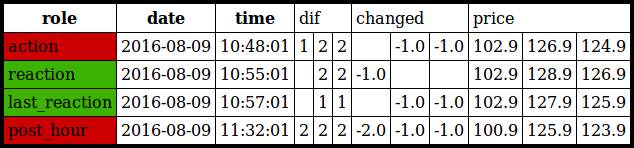
\includegraphics[width=0.6\textwidth]{Bilder/samr2.jpg}
	\caption{ein Auslöser - mehrere Reaktionen}
	\label{fig:SAMR}
\end{figure}
\autoref{fig:SAMR} beschreibt so einen Fall. Nur die spätere Reaktion kann die wahre Reaktion sein. Bei der Vorherigen ist die Anpassung bei Diesel höher als der Auslöser.

\item \textbf{mehrere Auslöser - eine Reaktion}\\
Der umgekehrte Fall, bei dem mehrere Änderungen eines Konkurrenten einer einzelnen Reaktion vorausgehen, lässt eine eindeutigere Entscheidung zu. In diesem Fall ist die letzte semantisch plausible Änderung des Konkurrenten der potentielle Auslöser. Angenommen, eine vorherige Änderung hätte die Reaktion ausgelöst, dann hätten alle noch folgenden Änderungen wiederum Reaktionen auslösen müssen. Es erfolgt jedoch offenbar nur eine Reaktion. Zudem ist diese Lösung wieder die sichere Variante. Bei den späteren Änderungen sind schon mehr Senkungen erfolgt, der Konkurrent hat also einen niedrigeren Preis. Die Reaktion stellt hier also einen verhältnismäßig niedrigen Schwellenwert wieder her. Sollte also der Fall eintreten, dass doch eine der früheren Änderungen der Auslöser war, und es wurde manuell eine weitere Senkung verhindert, so ist dies nicht nur ein von der Tankstelle gewollter Ausreißer, der auch als solcher bei der statistischen Auswertung keine Probleme bereiten sollte, sondern auch ein weniger kritischer Ausreißer, der die Wahl des Schwellenwertes nicht so stark beeinflusst.\\
Auch hier muss bei der Auswahl wieder berücksichtigt werden, dass eventuell mehrere Änderungen zusammen den Auslöser bilden. Die Auslöser werden deshalb von hinten durchiteriert. Handelt es sich bei dem aktuellen Auslöser um eine Änderung, bei der es bei den geänderten Kraftstoffsorten keinerlei Überschneidungen mit der Reaktion gibt, so kann diese Änderung übergangen werden. Das liegt daran, dass diese Änderung auch nicht eine erneute Änderung, wie oben beschrieben, hätte auslösen müssen. Sobald es eine solche Überschneidung gibt wird das semantische Kriterium überprüft. Wenn die Änderung mit dieser Überschneidung das semantische Kriterium noch nicht gänzlich erfüllt, können frühere hinzugenommen werden. Wieder dürfen dabei keine doppelten Änderungen einer Kraftstoffsorte entstehen, was bedeutet, dass wieder maximal zwei weiter Preisänderugnen als potentielle Auslöser dazugenommen werden können.
\begin{figure}[H]
	\center
	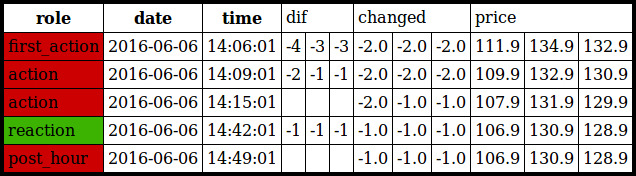
\includegraphics[width=0.6\textwidth]{Bilder/masr.jpg}
	\caption{mehrere Auslöser - eine Reaktion}
	\label{fig:MASR}
\end{figure}
In \autoref{fig:MASR} wird ein Beispiel für so einen Fall dargestellt. Von der Zeit her kommen alle Aktionen in Frage. Nach dem dritten Fall ist aber wahrscheinlich die letzte Aktion der wahre Auslöser. Hätten die Vorherigen Änderungen eine Reaktion erfordert, so hätte es für jede Nachfolgende ebenfalls eine Reaktion ausgelöst.

\item \textbf{mehrere Auslöser - mehrere Reaktion}\\
Die letzte Variante ist in der Umsetzung eine Kombination der vorherigen Fälle, was sich auch in der Begründung wiederspiegelt. Zunächst wird für die Kombination aller Auslöser untersucht, wieviele Reaktionen dadurch erklärt werden können. Dazu werden die Auslöser zu einem einzelnen künstlichen Auslöser zusammengefasst und dann die Reaktionen der Reihe nach addiert, solange das semantische Kriterium erfüllt bleibt. Sofern am Ende Reaktionen übrig bleiben, werden diese mit der selben Begründung wie im 2. Fall außer acht gelassen.\\

Die übrigen Reaktionen werden dann einzeln in rückwärtiger Reihenfolge untersucht, und gefundene Paarungen werden für die weitere Untersuchung gelöscht, sodass keine Doppelnennungen vorkommen können. Für die Betrachtung der jeweils letzten Reaktion, werden alle davorliegenden Auslöser gesammelt, und der 3. Fall wird angewendet. Das Entscheidungskriterium zugunsten des letzten möglichen Auslösers scheint hier außer Kraft gesetzt, denn spätestens ab der zweiten Iteration hatte es ja noch weitere spätere Reaktionen gegeben. Allerdings wurde für diese durch die rückwärtige Analyse bereits ein Auslöser gefunden oder es wurde bewiesen, dass es keinen semantisch möglichen Auslöser gibt, wodurch dieses Kriterium weiterhin gültig ist. Zudem gilt auch wieder, dass diese die sicherere Variante ist.\\

Wurden ein oder mehrere Auslöser für die aktuelle Reaktion gefunden, muss nur noch überprüft werden, ob weitere Reaktionen zwischen dem letzten der Auslöser und dieser aktuell letzten Reaktion liegen, die zusätzlich durch die gerade ausgewählten Auslöser erklärt werden können. Dabei kann es rein theoretisch wieder vorkommen, dass Auslöser, die zu einer späteren Reaktion passen, mit dieser gepaart und entfernt werden, obwohl sie eigentlich die Auslöser einer anderen, früheren Reaktion sind. Für diese Handhabung sprechen wieder die selben Gründe wie im 2. Fall. Wurde kein Auslöser gefunden, wird nur die gerade letzte Reaktion gelöscht.\\
\begin{figure}[H]
	\center
	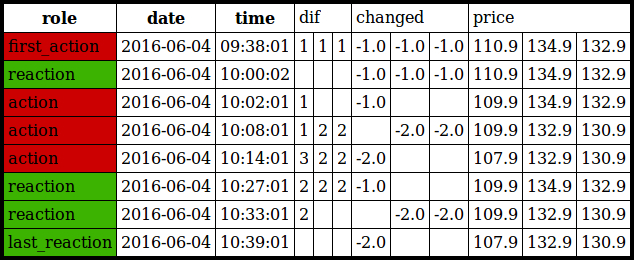
\includegraphics[width=0.6\textwidth]{Bilder/mamr3.jpg}
	\caption{mehrere Auslöser - mehrere Reaktion}
	\label{fig:MAMR}
\end{figure}
Das Reaktionsmuster in \autoref{fig:MAMR} ist ein relativ einfaches Beispiel so eines Falles, da die Reaktionen mittels der angepassten Werte eindeutig zu den Actionen gematched werden können. Davon kann jedoch nich immer ausgegangen werden.
\end{enumerate}

\section{Regeln spezifizieren}
Aus den gesammelten potentiellen Reaktionen sollen nun die in den Tools hinterlegten Regeln oder auch lediglich konsistente Verhaltensmuster abgeleitet werden. Dazu sollen die maximal zugelassene Preisabstände sowie die dazugehörigen Zeitintervalle erkannt werden. Letztlich muss dann über die ermittelten Regeln ermittelt werden, welche Tankstellen wirklich Konkurrenten sind. 

\subsection{Maximaler Preisabstand}
Die Verteilung der Preisdifferenz zweier Tankstellen ist das Hauptkriterium, auf welches sich die Klassifikation von Konkurrenz stützen wird. Wurde eine Regel und damit ein Schwellenwert für einen Konkurrenten hinterlegt, so sollte die Differenz nie lange über diesen Wert steigen. Es gibt zwei Möglichkeiten, wie eine Tankstelle auf die Änderung eines Konkurrenten entsprechend einer Regel reagieren kann. Entweder gar nicht, weil der Schwellenwert nicht überschritten wurde. Oder aber mit einer eigenen Preissenkung, wenn er überschritten wurde. Deshalb werden zwei verschiedene Differenzwerte unterschieden. Zum einen der Preisunterschied nach einer Änderung, auf die nicht reagiert werden musste. Der Maximalwert beschreibt hier den maximalen Abstand, auf den nicht reagiert werden musste. Gibt es eine Regel entspricht diese Differenz dem Schwellenwert. Zum anderen der Preisunterschied nachdem auf einen Konkurrenten reagiert werden musste. Für den Fall, dass es eine tatsächliche Reaktion und nicht nur eine Korrelation ist, sollte nach der reagierenden Preisänderung der Schwellenwert wieder hergestellt worden sein. Bei beiden Differenzen bestimmen die maximalen Werte den potentiellen Schwellenwert einer Regel. Um zu garantieren, dass genügend Daten für eine Analyse vorliegen, werden nur Konkurrenten analysiert, die mindestens ein Zehntel der Preisänderungen der untersuchten Tankstelle aufweisen.\\
Bei der Analyse dieser Werte werden die einzelnen Kraftstoffsorten zum ersten Mal komplett getrennt betrachtet. Werden bei einer Reaktion nicht alle Kraftstoffe angepasst, fällt diese Paarung für diese Sorte in die Kategorie, in der keine Reaktion notwendig war. Für jeden potentiellen Konkurrenten werden insgesammt je zwei Histogramme über die Preisunterschiede pro Kraftstoffsorte erstellt. Für das Histogramm über die Reaktionen müssen nur noch die Differenzwerte der gespeicherten Paarungen gebildet werden. Für das Histogramm über nicht erforderliche Reaktionen werden alle Preissenkungen des Konkurrenten ausgewählt, die nicht zu diesen Paarungen zählen. Jede dafür in Frage kommende Änderung wird noch einmal dahingehend überprüft, ob tatsächlich kein Pricing der untersuchten Tankstelle im anschließenden Zeitfenster zu finden ist. Durch das semantische Kriterium sind schließlich zeitlich korrelierende Anpassungen ausgeschlossen worden, weil sie keine Reaktionen darstellen. Es kann jedoch nicht mit Sicherheit gesagt werden, dass diese Änderung einen Preisabstand hergestellt hat, auf den nicht reagiert hätte werden müssen. Es könnte durchaus sein, dass eine Reaktion erforderlich gewesen wäre, hätte nicht ein anderer Konkurrent eine stärkere Reaktion bewirkt. Zudem müssen für die wirklich ignorierten Änderungen des Konkurrenten noch die zuletzt geltenden Preise der untersuchten Tankstelle ermittelt werden.\\
Die beiden Histogramme müssen dann für die Bestimmung des Maximalwertes zunächst zusammen betrachtet werden. Der dabei entstehende Maximalwert kann jedoch nicht sofort zum Schwellenwert gemacht werden. Es muss berücksichtigt werden, dass es durchaus noch sein kann, dass Tankstellen die Preise ohne Hilfe eines Tools anpassen oder zumindest die Anpassung selber noch manuell durchführen. Es kann also vorkommen, dass, obwohl eine Regel besteht, ab und zu dagegen verstoßen wird. Die Maximalwerte müssen also zunächst auf Ausreißer überprüft werden. Es wird also letztlich überprüft, ob die Häufigkeit, mit der ein entsprechender Wert auftritt, regelmäßig genug ist, um eine Vermutung von konkurrierendem Verhalten zu stützen. Diesbezüglich kann es durchaus vorkommen, dass zu einer Tankstelle eine Regel hinterlegt wurde, welcher nur sehr selten eine Reaktion erfordert. Ein Grund dafür könnte sein, dass der entsprechende Konkurrent selber in erster Linie auf die gerade untersuchte Tankstelle reagiert. Extremfälle dieser Art können nicht berücksichtigt werden, da ansonsten zu viele Ausreißer ebenfalls als Regel interpretiert werden würden.\\
Zusätzlich gilt es noch zu berücksichtigen, dass, sollte ein Wert zurückgewiesen werden, alle Differenzwerte,die diesen Schwellenwert gestützt hätten, zu Regelverstößen werden würden. Es gibt hierzu allerdings tankstellenübergreifend keine Erfahrungswerte, wie oft gegen Regeln verstoßen wird. Es ist durchaus möglich, dass sich dieser Faktor zwischen verschiedenen Unternehmen stark unterscheidet. Grundsätzlich sollte aber davon ausgegangen werden können, dass sich größententeils an Regeln gehalten wird, da diese Regeln im Allgemeinen einer ökonomischen Optimierung entstammen sollten, und Verstöße generell eine Gefahr bergen, Kunden zu verlieren.\\
Zuletzt ist es auch möglich für eine Tankstelle ihre Regeln auf bestimmte Zeit zu begrenzen, wodurch die Anzahl der zugehörigen Reaktionen auch deutlich geringer ausfallen kann. Diese drei Faktoren sprechen dafür, schon bei einer recht geringen Anzahl an unterstützenden Preismeldungen eine Regelmäßigkeit zu vermuten. Als Grenzwertfunktion wurde dafür diese Funktion gewählt:
\begin{center}
$ \frac{2}{\pi}*\arctan(2*\frac{x^2}{y})$\\
\end{center}
X stellt dabei die Häufigkeit dar, wie oft der entsprechende Differenzwert aufgetreten ist, und Y die Menge an Preismeldungen der Tankstelle im Allgemeinen. Als erste Richtlinie sollte der Grenzwert relativ zu der absoluten Menge der in diesem Zeitintervall liegenden Preisänderungen gewählt werden. Um die Häufigkeit des Wertes stärker zu gewichten, wird diese zunächst quadriert, bevor sie dann relativiert wird, damit bei moderat hohen Häufigkeiten eine unverhältnismäßig höhere absolute Anzahl an Preisänderugen nötig wäre, um diesen Wert zurückzuweisen. Angenommen, es würde einfach eine Prozenthürde von 10\% gewählt, so würde bei einer einzelnen entsprechenden Preisänderung aus zehn bereits ein Regel vermutet werden, wohingegen 9 aus 100 als Regel zurückgewiesen werden würden. Mit dem Arkustangens und den zusätzlichen Faktoren soll der errechnete Wert in einen Konfidenzwert zwischen 0 und 1 umgerechnet werden, der somit als Wahrscheinlichkeit interpretiert werden kann. Der Arkustangens garantiert dabei, dass die geringen Werte kaum verändert werden, wohingegen bei den hohen Werten der quadratische Faktor wieder etwas ausgeglichen wird. Die errechneten Konfidenzwerte lassen so trotz der verschieden großen Anzahlen an Preisänderungen zwischen den potentiellen Konkurrenten einen relativ guten Vergleich zwischen verschiedenen Regeln zu. Bei einem Maximalwert wird ab einer Häufigkeit, die einem Konfidenzwert größer als 0.5 entspricht, eine Regelmäßigkeit vermutet. Da es möglich ist, dass Tankstellen für einen Konkurrenten mehrere Regeln mit unterschiedlichen Schwellenwerten zu unterschiedlichen Zeiten erstellen, kann es durchaus vorkommen, dass neben dem maximalen Schwellenwert auch niedrigere Werte noch Regeln darstellen. Deshalb wird bei potentiellen Regeln zunächst überprüft, in welchem Zeitfenster sie gültig sind. Solange noch Zeitslots existieren, in denen noch keine Regel befolgt wird, werden die nächst niedrigeren Differenzwerte untersucht. 

\subsection{Zeitintervall}
Für jeden möglichen Maximalwert müssen nun die Zeitintervalle ermittelt werden, in denen dieser Wert auftritt. Sie definieren das Zeitfenster der Regel. In einem ersten Ansatz sollten die Regeln zunächst von den Zeitintervallen ausgehend erstellt werden, statt zunächst die Schwellenwerte zu errechnen. Die Daten sollten dafür rekursiv in immer kleinere Zeitintervalle aufgespalten werden. Anschließend sollte für jedes Intervall aus den darin liegenden Daten die Schwellenwerte, wie oben beschrieben, errechnet werden. Zuletzt sollten die Slots mit gleichen Abstandswerten zusammengefügt werden um wieder größere Intervalle zu bilden. Dies hat dazu geführt, dass bereits beim Versuch, die Daten nach einzelnen Wochentagen oder Stunden zu spalten, zu wenig Daten für die einzelnen Intervalle zur Verfügung standen, um halbwegs sichere Aussagen treffen zu können. Auch sind nicht so hochfrequente Konkurrenzmuster gänzlich unerkannt geblieben. In den zu Testzwecken zur Verfügung stehenden Regeln gibt es zwar nur wenige Einzelfälle, bei denen überhaupt eine zeitliche Unterscheidung von Schwellenwerten getroffen wurde. Es muss aber auch hier berücksichtigt werden, dass diese Testwerte nicht umbedingt repräsentativ für den ganzen Kraftstoffmarkt sind und andere Tankstellen durchaus feinere Unterscheidungen treffen könnten. Aus diesem Grund musste dieser Ansatz verworfen werden.\\
Stattdessen wird zunächst ein Tage- und Stundenübergreifend gültiger Schwellenwert vermutet. Deswegen werden die Differenzhistogramme wie oben beschrieben über den gesamten Zeitraum gebildet. Anschließend wird ermittelt, in welchen Zeitintervallen dieser Maximalwert auftritt. Hierbei wird nur einzeln entweder nach ganzen Tagen oder nach Stunden unterschieden. Es könnte sein, dass detailliertere Regeln für kleinere Stundeunintervalle an einzelnen Tagen existieren. Es ist aber relativ unwahrscheinlich, dass so eine feine Unterscheidung allzu häufig getroffen wird. Schließlich sollte es für jede weitere Aufsplittung eine ökonomische Rechfertigung geben. Es ist unwahrscheinlich, dass Kunden die Tankstellenpreise so genau verfolgen, dass sie die Preisabstände zu jeder Tages- und Uhrzeit kennen. Es müsste also ein gänzlich andere Art von Kundenaufkommen für diese speziellen Intervalle vermutet werden, die anderer Preisabstände rechtfertigen. Und selbst, wenn solche Unterschiede weit verbreitet wären, wäre eine detailliertere Analyse aufgrund der Dichte der Daten einfach kaum möglich.

\subsubsection{Potentielle Zeitintervalle ermitteln}
Dafür müssen zunächst alle möglichen Zeitslots für Tage und Stunden ermittelt werden. Dies sind die Zeiten, zu denen jeweils die untersuchte Tankstelle und der Konkurrent gleichzeitig geöffnet haben. Wie eben angesprochen werden nur die einzelenen Tage und tageübergreifend eine Stundenanzahl ermittelt. Es würden also auch keine unterschiedlichen Öffnungszeiten an Wochenenden berücksichtigt werden. Es gilt dann die längste Öffnungszeit der Woche. Die Öffnungszeiten der Tankstellen stehen in dem Datensatz von Tankerkönig nicht zur Verfügung. Allerdings reicht es auch, zu ermitteln, in welchen Zeitslots beide Tankstellen Preisänderungen durchführen, da diese Slots ohnehin auch nur die Zeitslots sind, bei denen Daten zur Verfügung stehen. Es ist außerdem besonders wichtig, dass jeder Zeitslot auch Daten hat, an denen er untersucht werden kann, da so lange weitere Schwellenwerte überprüft werden, bis alle Slots belegt sind. Auch hier müssen deswegen wieder Ausreißer berücksichtigt werden. Bei beiden Kategorien - Tagen und Stunden - werden die \textit{Öffnungszeit} für die in der Analyse betrachteten Tankstellen getrennt ermittelt und anschließend die der untersuchten Tankstelle mit dem jeweiligen Konkurrenten kombiniert.\\
Zur Bestimmung der geöffneten Tage wird der Mittelwert an Preisänderungen berechnet. Dabei fließen nur Tage in die Berechnung mit ein, an denen überhaupt Änderungen stattfinden. Ein Tag muss ein Zehntel dieses Mittelwertes überschreiten, um als gültiger Tagesslot zu gelten. Das ist notwendig, um einerseits Ausreißer auszuschließen und andererseits gewährleisten zu können, dass die Analyse des jeweiligen Maximalwertes für jeden Tag genügend zugrunde liegende Daten aufweist. Die Bestimmung der Stunden läuft bis dahin äquivalent ab. Allerdings müssen hier neben den positiven Ausreißern, also Preisänderungen zu Zeiten, in denen die Tankstelle eigentlich nicht geöffnet ist, aber aus irgendwelchen Gründen trotzdem Preise geändert werden auch negativ Ausreißer, also Zeiten in denen die Tankstelle geöffnet hat aber nur sehr wenige oder gar keine Preissenkungen vornimmt, berücksichtigt werden. Auch hier werden die Erhöhungen herausgenommen, da diese oftmals zu Randzeitpunkten wie zu Beginn oder am Ende einer Öffnungsperiode stattfinden und dabei öfters aus der tatsächlichen Öffnungszeit herausfallen. Für jede Stunde werden bei der Entscheidung zusätzlich jeweils die drei vorherigen und folgenden Stunden berücksichtigt. Für das vorangegangene und nachfolgende Intervall werden jeweils die Stunden gezählt, bei denen der Grenzwert von einem Zehntel vom Mittelwert überschritten wurde. Wird bei der betreffenden Stunde selber dieser Wert überschritten, so wird das Maximum dieser beiden Randintervalle gewählt und für die Entscheidung wird überprüft, ob mindestens zwei der drei Stunden ebenfalls diesen Wert überschreiten. Wird der Wert für die Stunde selber nicht erreicht, so wird das Minimum der Randintervalle dem gleichen Test unterzogen. Dieses Verfahren hat den Hintergrund, dass bei den Testtankstellen innerhalb der Öffnungszeiten Intervalle von zwei Stunden auftreten können, zu denen es kaum oder selten auch mal keine Änderungen gibt. Hier konnte auch repräsentativ getestet werden, da die Öffnungszeiten generell öffentlich zugänglich sind. Dieses Verfahren ermöglicht es diese Stunden trotzdem in die Analyse mit einzuschließen und gleichzeitig die Ränder nicht zu vergrößern. Zwar gibt es für diese auf diese Weise miteingeschlossenen Stunden keine Daten, was aber nicht problematisch ist, weil diese Fälle im weiteren Verlauf auch wieder berücksichtigt werden.

\subsubsection{Konkrete Zeitintervalle für Regeln definieren}
Wenn die möglichen Zeitslots feststehen, muss für die Schwellenwerte bezüglich eines Konkurrenten ein Gültigkeitsbereich definiert werden. Diese Slots ergeben sich durch die Verteilung derjenigen Reaktionen und ignorierten Preisänderungen, die exakt diesen gerade untersuchten Maximalwert generiert haben. Deshalb wird noch einmal ein Tages- sowie Stundenhistogramm für genau diejenigen Änderungen erstellt, die in diese Kategorie fallen. Es kann sein, dass dieser Schwellenwert nicht in jedem Slot vorkommt. Diejenigen Slots, bei denen nicht genügend Reaktionen oder ignorierten Preisänderungen mit Differenzen in dieser Höhe existieren, sind Kandidaten für eine weitere schwächere Regel.\\
Damit ein Zeitslot den aktuellen Schwellenwert zugewiesen bekommt, müssen ähnliche Probleme wie auch schon bei der Analyse der generell verfügbaren Slots, bedacht werden. Bei der Festlegung der Tage sind die Werte noch dicht genug, dass vom Ablauf her das gleiche Verfahren durchgeführt wird, mit dem einzigen Unterschied, dass diesmal nicht alle Preisänderungen in Frage kommen, sondern nur die dem aktuellen Schwellenwert zugehörigen. Wegen dieser Einschränkung der Datenmenge muss die Analyse bei den Uhrzeiten noch einmal abgewandelt werden. Das Pricingverhalten ist auch bei normalem, regelkonformem Verhalten hier bereits größeren Schwankungen unterlegen. Der Grenzwert, ab dem ein Slot belegt wird, ist deshalb abhängig von der Relation, der in diesem Slot liegenden Änderungen, welche die gerade getesteten Höhe aufweisen, zu der Gesammtheit aller in diesem Slot liegenden Preisänderungen. Der Anteil sollte 10\% nicht unterschreiten. Auch hier müssen wieder die Schwankungen berücksichtigt werden. Um nicht stark fluktuierende Regeln zu generieren, das heißt im Extremfall solche, die jeweils immer nur für einzelne Stunden gültig sind, wird die Mindestgültigkeitsdauer einer Regel auf 3 Stunden gesetzt. Daraus ergibt sich, dass sowohl einzelne Slots zusätzlich aufgenommen, als auch trotz hoher Werte zurückgewiesen werden können. Für die Umsetzung wird ein fünf Slots großer Kernel über die Liste der Uhrzeiten laufen gelassen wird, der die Belegung des einzelnen Slots im Zentrum danach auswählt, ob mehr oberschwellige oder mehr unterschwellige Werte in diesem Kernel liegen. Nach diesem Schritt sind für jeden Konkurrenten die möglichen Regeln eindeutig definiert.

\subsection{Klassifikation Konkurrenz}
Das Finden einer Regel bedeutet allerdings noch nicht die Existenz einer Konkurrenz. Bei der Entscheidung zugunsten einer Regel wurden schließlich nicht nur Reaktionen sondern auch die ignorierten Preisänderungen berücksichtigt. Der Konfidenzwert der Regel gibt nur an, dass, sollte überhaupt eine Regel zu dem jeweiligen Konkurrenten bestehen, dann sollte dieser Abstandswert mit der Sicherheit dieses Wertes eine Regel darstellen. Es kommt deshalb häufig vor, dass zwar hohe Sicherheiten bezüglich einer Regel bestehen, diese aber keine oder kaum Reaktionen erzeugt, weil der entsprechende potentielle Konkurrent eben kein wirklicher Konkurrent ist. Die hohe Sicherheit kommt dann dadurch zustande, dass der Abstandswert häufig zustande gekommen ist, ohne dass die untersuchte Tankstelle darauf reagieren wollte.\\
Um eine andere Tankstelle als Konkurrenten zu klassifizieren, muss also ein anderer Konfidenzwert berechnet werden. Der Einfachheit halber wurde hier der Anteil der Preissenkungen der untersuchten Tankstelle genommen, welcher durch die ermittelten Regeln gegenüber einem Konkurrenten hervorgerufen worden sein könnte. Das ist die Summe der Reaktionen jeder einzelnen Regel geteilt durch die Anzahl an Preissenkungen der untersuchten Tankstelle. Das hat den Hintergrund, dass ein tatsächlicher Konkurrent auch häufiger Reaktionen hervorrufen sollte, um als solcher gelten zu können. Wenn es trotzdem Fälle gibt, in denen Konkurrenten im System hinterlegt wurden, die kaum Reaktionen erzeugen, dann wäre es auch nicht besonders schädlich diese nicht als Konkurrenten zu klassifizieren, da die so falsch erklärten Preissenkungen sich auf einige wenige belaufen würden. Der Threshold wird dabei zunächst relativ niedrig auf drei Prozent gesetzt, um möglichst alle Konkurrenten zu erkennen. Die Erkennungsrate auf diese Weise hochzutreiben bringt natürlich eine hohe Wahrscheinlichkeit von $\alpha$ -Fehlern mit sich, also Fälle, in denen Konkurrenzen vermutet werden, wo eigentlich gar keine existieren. Diese Art von Fehlannahme hat auch noch weitere begünstigende Faktoren. Es ist in dieser Version noch nicht ausgeschlossen, dass für eine Reaktion verschiedene Auslöser von verschiedenen Tankstellen jeweils in deren Regeln mitgezählt werden. Die Summe der ermittelten Reaktionpaarungen über alle Konkurrenten hinweg kann also deutlich größer sein als die Anzahl der Reaktionen an sich. Die Auswirkungen dieser Faktoren werden in der folgenden Diskussion der Ergebnisse dargestellt.
%ergebnisse.tex
\chapter{Ergebnisse}
\label{sec:Ergebnisse}

Bei einer üblichen Klassifikation im Bereich des maschinellen Lernens mit ausreichend klassifizierten und zudem repräsentativen Trainingsdaten würde man hier nun eine Trainings- und Testphase durchführen. Das bedeutet die Trainingsdaten würden in ein Traningsset und ein Testset aufgeteilt werden. Man würde dann die im Algorithmus verwendeten Parameter anhand des Trainingssets optimieren und dann mit Hilfe des Testsets die allgemeine Performance überprüfen. Wie schon bei der Analyse der Daten festgestellt wurde, ist die Menge der zur Verfügung stehenden Regelsätze weder ausreichend noch repräsentativ für den ganzen Markt. Zur Verfügung stehen die Regelsätze von neun verschiedenen Tankstellen, die alle von einem einzelnen Preishoheitsinhaber gesteuert werden. Es gibt verschiedene Ansätze, wie in diesen Fällen vorgegangen werden kann, um dieses Format trotzdem beibehalten zu können. Es könnte zum Beispiel künstlich ein dem Markt entsprechendes Setup simuliert werden, welches genügend Trainingsdaten erzeugt. Das würde bedeuten, künstlich Tankstellen mit Konkurrenten und Regeln zu erzeugen, authentisches Verhalten zu implementieren und somit einen neuen Datensatz zu erzeugen, anhand dessen vernünftig trainiert werden könnte. Abgesehen davon, dass dafür einige Parameter aus dem originalen Datensatz benötigt würden, um einen authentischen künstlichen Markt zu generieren, würde der Aufwand dafür den Rahmen dieser Arbeit überschreiten. Deshalb werden hier einfach die vorhandenen Daten verwendet.  

\section{Diskussion}
Auch wenn das Ziel nicht war, alle existierenden Regeln zu erkennen, so bieten diese Regeln doch eine gute Grundlage, die generierten Ergebnisse dieses ersten Ansatzes systematisch zu diskutieren. Statt die übliche Optimierung der Parameter  anzustreben soll hier eher genauer dargelegt werden, wie sich verschiedene Einstellungen auf den weiteren Verlauf und die letztlichen Ergebnisse des Programmes auswirken. Dazu wird zunächst ein Testlauf mit den \textit{default} Werten duchgeführt. Dann werden die Ergebnisse und verschiedene andere Faktoren in Vier-Felder-Tafeln dargestellt, um genauer auf die veschiedenen Formen von Fehlklasifikationen eingehen zu können. Zu den besonders auffälligen Werten werden dann Hypothesen aufgestellt, was die Ursachen für diese Ergebnisse sein könnten. Diese Hypothesen werden dann mittels weitere statistiken untermauert werden.

\begin{figure}[!ht]
	\caption{Konkurrenten Entscheidungsgenauigkeit}
	\hspace*{\fill}%
		\subfloat[Default Einstellung]{\label{fig1:DE}
			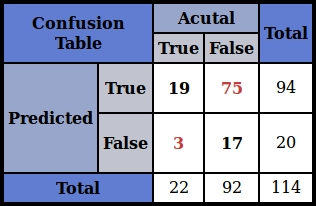
\includegraphics[width=0.3\textwidth]{Bilder/default_comp_overall_acc.jpg}}
		\hfill
		\subfloat[Erhöhte Mindestzahl an potentiellen Konkurrenten]{\label{fig1:EM}
			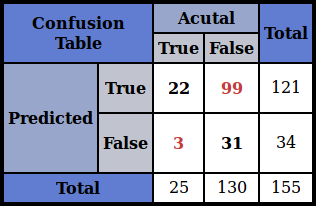
\includegraphics[width=0.3\textwidth]{Bilder/n_val_comp_overall_acc.jpg}}
		\hfill
		\subfloat[Differenz]{\label{fig1:D}
			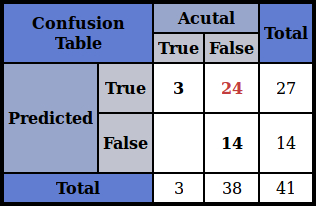
\includegraphics[width=0.3\textwidth]{Bilder/n_val_comp_dif_acc.jpg}}
	\hspace*{\fill}%
	\label{fig:KE}
\end{figure}

Wie in \autoref{fig:KE}\subref{fig1:DE} zu sehen, ist die Zahl der $\beta$-Fehler relativ gering. Es werden also fast alle Konkurrenten erkannt. Bei den nicht erkannten Konkurrenten handelt es sich um Fälle, in denen sich die Anzahl der zu den jeweiligen Regeln gehörenden Reaktionen auf maximal 9 beziehungsweise 2\% beschränkt. Auf die drei Monate verteilt wäre dies nicht einmal eine Reaktion pro Woche. Die Tabelle beinhaltet allerdings nur die untersuchten Tankstellen, also nicht jene, die schon bei der Auswahl der potentiellen Konkurrenten über die Abstandsbestimmung aus dem Raster fallen. Die default Einstellung hat als Abstandsobergrenze 5km, welche sich jeweils verdoppelt, wenn die Mindestanzahl von 5 Konkurrenten nicht erreicht worden ist. Bei diesen Parametern beläuft sich die Anzahl der nicht erfassten Konkurrenten auf drei. Erhöht man die Mindestzahl der Konkurrenten auf 10, so sinkt dieser Wert auf null herab. Allerdings werden bei dieser Einstellung wie in \autoref{fig:KE}\subref{fig1:EM} und \subref{fig1:D} zu sehen insgesamt 41 Tankstellen mehr untersucht, wovon 24 fälschlicherweise auch als Konkurrenten klassifiziert werden. Diese Einstellung würde sich demnach nur lohnen, wenn die Anzahl der $\alpha$-Fehler deutlich reduziert werden kann. Diese hohe Zahl an vermeintlich erkannten Konkurrenten hat vermutlich verschiedene Ursachen. Zunächst sollte natürlich der Konfidenz-Threshold für Konkurrenten betrachtet werden.

\begin{figure}[!ht]
	\center
	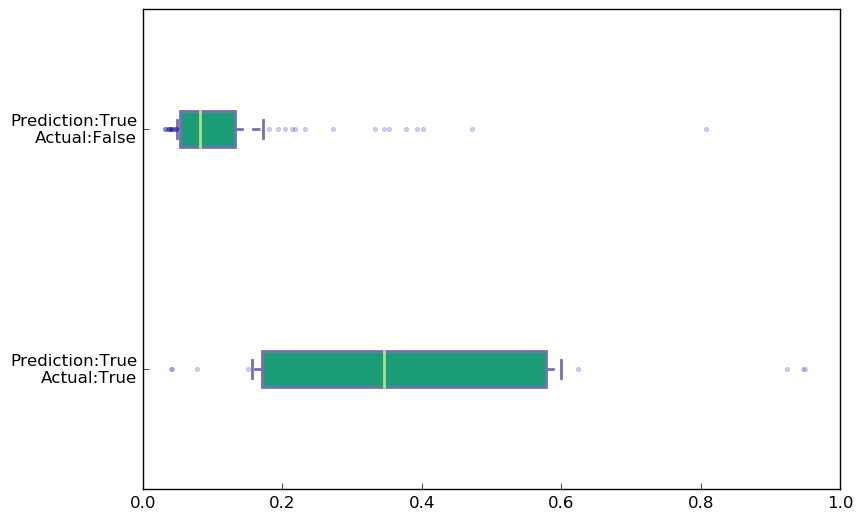
\includegraphics[width=0.6\textwidth]{Bilder/comp_conf_boxplot.png}\\
	\caption{Konkurrenz-Konfidenz-Verteilung}
	\label{fig:KKV}
\end{figure}

\autoref{fig:KKV} zeigt Boxplots der jeweiligen Konfidenzwerte der Konkurrenten und unterscheidet zwischen tatsächlichen Konkurrenten und den fälschlicherweise als Konkurrenten erkannten Tankstellen. Die beiden Fälle, in denen der Algorithmus die Tankstelle nicht als Konkurrenten klassifiziert, sind nicht aufgeführt, da hier alle Konfidenzwerte unter der Untergrenze von 3\% liegen. Würde man den Threshold auf 15\% erhöhen, könnte man in diesem Testszenario die Anzahl der $\alpha$-Fehler um 75\% reduzieren. Allerdings würden dann auch circa 15\% der richtig erkannten Konkurrenten zu $\beta$-Fehlern werden. Die Wahl des Wertes sollte jedoch eher inhaltlich begründet werden, als an den letztendlichen Ergebnissen dieses Tests. Der durchschnittliche Konfidenzwert beträgt bei den tatsächlichen Konkurrenten in etwa 35\% und bei allen anderen ungefähr 10\%. Die 10\% sind demnach so etwas wie eine zufällige Korrelation, die im Mittel zwischen jeder Paarung von Tankstellen existiert. Der Wert fällt allerdings höchstwahrscheinlich ein um einiges höher aus, weil nur benachbarte Tankstellen in diesen Wert eingehen, bei denen zu einem nicht geringen Anteil auch wirklich stark korrelierende Paarungen existieren, die zwar nicht direkt kausal verknüpft sind, sich aber indirekt über dritte Tankstellen parallel verhalten. Anders wären die oberen 10\% der $\alpha$-Fehler in \autoref{fig:KKV} kaum zu erklären.\\
Statistisch gesehen sollte der Threshold dann so gelegt werden, dass signifikante Ausreißer der zufälligen Korrelation zu Konkurrenten erklärt werden. Problematisch bei so einem Ansatz ist, dass die zufällige Korrelation und die kausal bedingte Korrelation so nahe beieinanderliegen, dass sich statistisch vermutlich kein eindeutiger Grenzwert ermitteln lässt. Damit ist gemeint, dass der obere Grenzwert für Ausreißer einer zufälligen Korrelation höher liegt als die Untergrenze für negativ Ausreißer einer kausalen Korrelation. Der Threshold sollte dann in der Schnittmenge liegen, wobei die stärkere Orientierung zu einem der Grenzwerte für Ausreißer eine bestimmte Art von Fehler stärker begünstigt. Der default Wert von 3\% neigt sehr stark dazu, $\beta$-Fehlern zu vermeiden und generiert damit große Mengen an $\alpha$-Fehlern. Erhöht man den Wert auf 10\%, werden 3 $\beta$-Fehler mehr erzeugt während die $\alpha$-Fehler um 42 reduziert werden, was in der Summe der Fehler natürlich eine Steigerung der Performanz bedeuten würde. Alles in allem ist dieser Wert in dieser Form für eine letztendliche Klassifikation nicht besonders gut geeignet.\\
Da dieser Konfidenzwert sehr stark von den erkannten Regeln abhängig ist, können sich auch Veränderungen dort auf die allgemeine Performanz bei den Konkurrenten auswirken. Auch für die Regeln gibt es wieder einen Konfidenzwert, der analysiert werden kann.

\begin{figure}[!ht]
	\center
	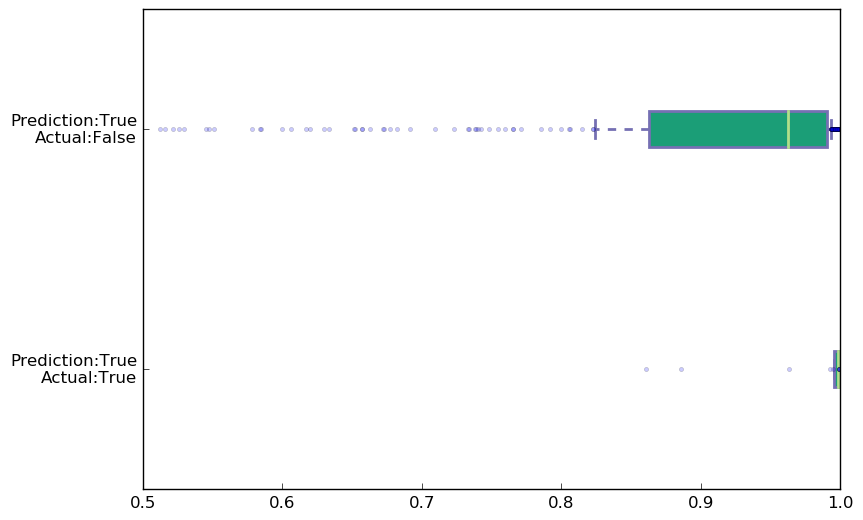
\includegraphics[width=0.6\textwidth]{Bilder/rule_conf_boxplot.png}
	\caption{Regel-Konfidenz-Verteilung}
	\label{fig:RKV}
\end{figure}

Die Idee dieses Wertes war eigentlich, dass nicht die Höhe klassifiziert, ob tatsächlich eine Regel besteht, sondern die Anteile an Reaktionen und ignorierten Preisänderungen, die den Abstand der potentiellen Regel wieder hergestellt beziehungsweise so belassen haben. Hohe Anteile von ignorierten Preisänderungen sollten darauf hindeuten, dass generell keine Konkurrenz besteht und auch nicht weiter nach Regeln gesucht werden muss, während hohe Anteile an Reaktionen eine tatsächliche Regel andeuten sollten. 
Schaut man sich jedoch die Verteilung in \autoref{fig:RKV} an, dann sind die Werte für tatsächliche Regeln eindeutig signifikant höher als bei nicht regelgemäßem Verhalten. Das liegt daran, dass bei nicht regelgemäßem Verhalten die Abstandswerte eine größere Streuung aufweisen. Bei einer Regel sind die Abstandswerte in gewisser Weise nach oben beschränkt, da höhere Abstände sofort wieder auf den der Regel entsprechenden Abstand herabgesetzt werden. Wenn keine Regel vorliegt, verteilen sich die Abstandswerte entsprechend der Höhe der Preisschwankungen auf wenige, aber trotzdem mehrere Werte. Dadurch wird der Eindruck erweckt, es würden mehrere Regeln bestehen. Dieses Verhalten wird auch noch in einigen weiteren Werten sichtbar. Zum Beispiel ist dadurch auch die mittlere Anzahl an Regeln pro Konkurrent bei den tatsächlichen Regeln deutlich niedriger.\\

\begin{figure}[!ht]
	\caption{Regel Treffergenauigkeit}
	\hspace*{\fill}%
		\subfloat[Default Einstellung]{\label{fig1:D}
			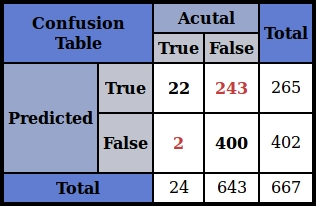
\includegraphics[width=0.3\textwidth]{Bilder/default_rule_overall_acc.jpg}}
		\hfill
		\subfloat[Erhöhte Untergrenze bei dem Konfidenzwert für Regeln]{\label{fig1:ERKU}
			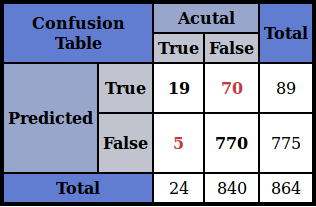
\includegraphics[width=0.3\textwidth]{Bilder/rule_conf_overall_rule_acc.jpg}}
	\hspace*{\fill}%
	\label{fig:RT}

	\bigskip

	\caption{Mittlere Anzahl an Regeln pro Konkurrent}
	\hspace*{\fill}%
		\subfloat[Default Einstellung]{\label{fig1:DMRpK}
			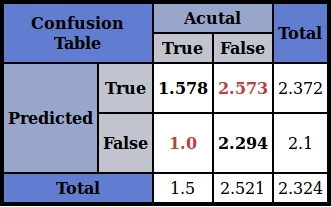
\includegraphics[width=0.3\textwidth]{Bilder/default_avg_num_rules.jpg}}
		\hfill
		\subfloat[Erhöhte Untergrenze bei dem Konfidenzwert für Regeln]{\label{fig1:EMRpK}
			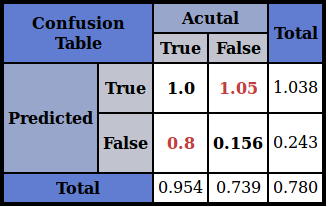
\includegraphics[width=0.3\textwidth]{Bilder/rule_conf_avg_num_rules.jpg}}
	\hspace*{\fill}%
	\label{fig:MRpK}
\end{figure}

\autoref{fig:RT} und \autoref{fig:MRpK} unterstützen diese Erklärung. Hier wurde der Grenzwert für Regeln von dem default Wert 0.5 auf 0.99 erhöht, was sich in der Verteilung der Konfidenzwerte im obigen Boxplot als ein guter Trennwert herausgestellt hat. Die Anzahl der fehlerhaften Regeln nimmt stark ab, weil einfach generell die Anzahl der Regeln abnimmt. Dies hat auch einen positiven Effekt auf die Fehler bei der Klassifikation der Konkurrenten.\\
Andere Möglichkeiten, diesen Umstand auszunutzen, wären demnach, die Anzahl an Regeln per se auf eine einzelne pro Konkurrent zu beschränken oder den Konfidenzwert für Konkurrenten durch die Anzahl an Regeln zu teilen. Alle diese Eingriffe senken die Anzahl der $\alpha$-Fehler bei den Konkurrenten erheblich und verursachen nur eine geringe Anzahl an neuen $\beta$-Fehlern. Das liegt zu großen Teilen aber auch daran, dass in den Testdaten fast nur einzelne Regeln vertreten sind. Bei mehreren Regeln pro Konkurrenten verteilen sich die Abstandswerte auch, hier dann auf die verschiedenen Regeln, und sind somit auch stärker gestreut. Das führt schon bei den wenigen Fällen im Testset mit zwei Regeln für einen Konkurrenten dazu, dass diese nicht mehr erkannt werden. Diese Art von Anpassung würde also nur Sinn machen, wenn man davon ausgehen könnte, dass generell nur eine Regel pro Konkurrent anzunehmen ist.\\
Ein anderer Faktor, der sich bei den $\alpha$-Fehler stark von den tatsächlichen Konkurrenten abhebt, sind die Ausnahmen der Regeln, also die Preisabstände, die oberhalb der Regel innerhalb des relevanten Intervalls auftreten. Dadurch, dass bei mehreren Regeln die jeweiligen Zeitintervalle kleiner sind, bestehen jeweils immer große Intervalle für weitere niedrigere Regeln. In diesen Intervallen, wo prinzipiell Regeln gelten können, welche aber erst von niedrigeren Regeln belegt werden, können dann auch vermehrt höhere Abstände auftreten als bei einer einzelenen Regel über dem ganzen Intervall. Gerade bei Verhalten, welches sich nicht an Regeln orientiert, sind die Werte stark über den ganzen Zeitraum hinweg gestreut und führen so bei kleinen Regelintervallen zu vielen Ausnahmen, die bei jeder weiteren Regel mehr werden. Bei mehreren Regeln und regelkonformem Verhalten sind zwar auch die Intervalle der einzelnen Regeln kleiner, aber die Abstandswerte beschränken sich weitgehend, das heißt bis auf einzelne Ausreißer, auf das für die Regel gültige Intervall. Deshalb bleibt hier auch ein Unterschied erhalten, wenn man den Mindestkonfidenzwert für Regeln erhöht und so generell weniger Regeln klassifiert werden.\\

\begin{figure}[!ht]
	\center
	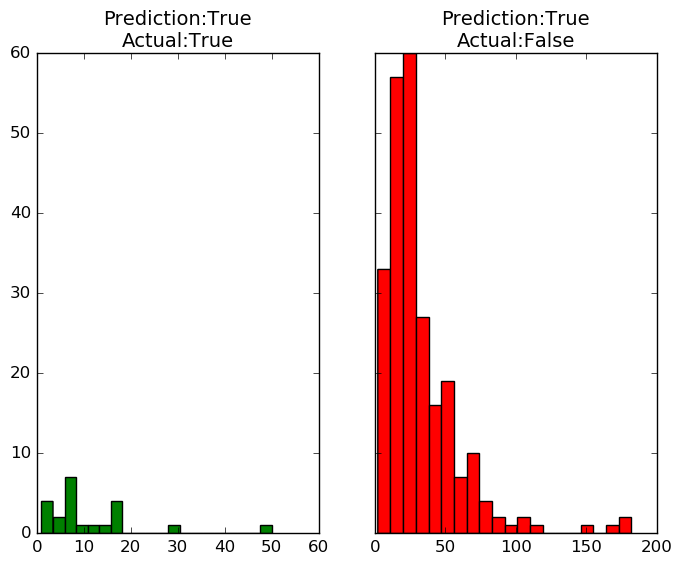
\includegraphics[width=0.6\textwidth]{Bilder/exception_hist.png}\\
	\caption{Regel-Ausnahmen-Verteilung}
	\label{fig:RAV}
\end{figure}

\autoref{fig:RAV} zeigt den starken Unterschied bei den Ausnahmen zwischen tatsächlichen und vermeintlichen Regeln. Die Ausnahmen in diesen Konfidenzwert mit einzuberechnen sollte die Klassifikation hier also deutlich verbessern.\\
Vor dem Hintergrund wird auch ersichtlich, dass es wichtig ist, sich die Intervalle der Regeln genauer anzuschauen. In Testdaten gelten die Regeln immer an allen Tagen, weshalb bei den Tagesintervallen keine neuen Erkenntnisse zu erwarten sind. Die Güte der Klassifikation an sich ist auch nicht besonders aussagekräftig. Es wurden zwar für die Statistik nur die Regeln ausgewählt, wo letzlich auch eine Konkurrenz vermutet wurde. Allerdings ist es bei der Höhe der $\alpha$-Fehler bei den Konkurrenten und den Regeln dann auch nicht verwunderlich, dass bei den Stunden hier erhebliche Mengen an Fehlern bestehen. Interessant sind Werte, die helfen, Regeln aufgrund von unplausiblen Intervallen zurückzuweisen, um eben die Klassifikation von Regeln zu verbessern. Hier sind vor allem zwei Faktoren interessant.
\begin{figure}[!ht]
	\caption{Generelle Stunden Statistiken}
	\hspace*{\fill}%
		\subfloat[Stunden Treffgenauigkeit]{\label{fig1:ST}
			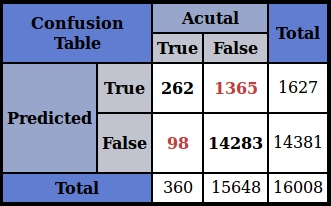
\includegraphics[width=0.3\textwidth]{Bilder/default_hour_overall_acc.jpg}}
		\hfill
		\subfloat[Mittlere Anzahl an Stunden pro Regel]{\label{fig1:MSpR}
			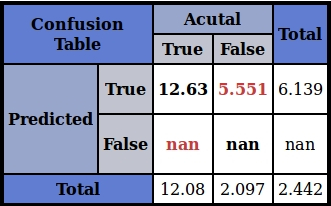
\includegraphics[width=0.3\textwidth]{Bilder/default_avg_num_hours.jpg}}
	\hspace*{\fill}%
	\label{fig:GSS}

	\bigskip

	\caption{Angepasste Stunden Statistiken}
	\hspace*{\fill}%
		\subfloat[Anteil an Regeln mit geänderten Stunden]{\label{fig1:ARgS}
			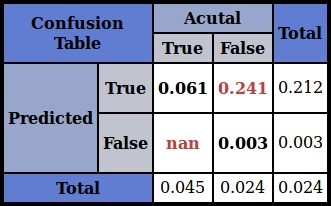
\includegraphics[width=0.3\textwidth]{Bilder/default_avg_hours_changed.jpg}}
		\hfill
		\subfloat[Mittlere Anzahl an geänderten Stunden pro Regel]{\label{fig1:MgSpR}
			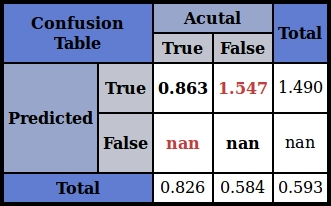
\includegraphics[width=0.3\textwidth]{Bilder/default_avg_num_hours_changed.jpg}}
	\hspace*{\fill}%
	\label{fig:GS}
\end{figure}
\autoref{fig:GSS} zeigt zum einen, dass sich die tatsächlichen Regeln von den fälschlicherweise erkannten erheblich in der Anzahl an Stunden pro Intervall unterscheiden. Zum anderen wurde bei den Stunden gerade wegen den teilweise unregelmäßigen Verteilungen auch bei tatsächlichen Regeln eine Art Smoothing verwendet, was einzelne Ausreißer in der Klassifikation an die Werte der Umgebung angepasst hat. Das sollte in erster Linie dazu führen, dass einzelne Regeln begünstigt werden sollten und nicht allzu kleine Intervalle entstehen. Zudem besteht bei der default Einstellung eine Mindestgröße für Regeln nach der sich der Filter für das Smoothing richtet. Die Werte für die tatsächlichen Regeln lassen vermuten, dass dies in diesem Fall auch hilfreich ist. Die nan Werte kommen zustande, weil bei zurückgewiesenen Regeln nicht das Zeitintervall überprüft wird, was dazu führt, dass in diesen Felder eventuell durch null geteilt werden würde.\\
Wie in der \autoref{fig:GS} zu sehen ist, wurden in wenigen Fällen einige negative Ausreißer mit ins Intervall aufgenommen, was zu einer Durchschnittslänge von 12.63 geführt hat. Dabei sollte wieder berücksichtigt werden, dass kleinere Intervalle auch kaum in den Testdaten vorkommen. Die Statistik zeigt aber auch, dass das Smoothing bei fehlerhaft erkannten Regeln viel häufiger und gleichzeitig auch absolut mehr Stunden in das Intervall mit aufgenommen hat. Trotzdem wurden dadurch im Durchschnitt mit 5.5 Stunden nur sehr kurze Intervalle erkannt. Bei 1.5 angepassten Stunden pro falscher Regel sind also mehr als ein Viertel der Stunden wegen ihrer Umgebung trotzdem in das Intervall aufgenommen worden. Das Verfahren ist also in dieser Form noch nicht besonders hilfreich. Es sollte ein anderes Vorgehen entworfen werden, was größere Intervalle noch stärker unterstützt und bei starker Streuung auch die Möglichkeit besitzt, eine Regel zurückzuweisen. Das würde zwar wahrscheinlich auch wieder die existierenden Konkurrenten mit mehreren Regeln mit jeweils nur wenigen Stunden benachteiligen, allerdings sollte eine Aufteilung in verschiedene Regeln an einem Tag auch inhaltlich begründet sein. Man sollte annehmen können, dass bei kurzen Intervallen ein besonderes Augenmerk auf diese Konkurrenz gelegt wurde und dass in diesem Intervall auch einige Änderungen stattfinden, die der gesonderten Anpassung bedürfen. Es sollte dort also von einer geringeren Streuung ausgegangen werden können. Ab einem gewissen Punkt, also kurze Intervalle mit starker Streuung, wäre es auch schlicht nicht mehr möglich und inhaltlich sinnvoll begründbar, diese als gesonderte Regeln zu identifizieren.
\begin{figure}[!ht]
	\caption{Erhöhte Mindestanzahl an Stunden pro Regel}
	\hspace*{\fill}%
		\subfloat[Anteil an Regeln mit geänderten Stunden]{\label{fig1:EARgS}
			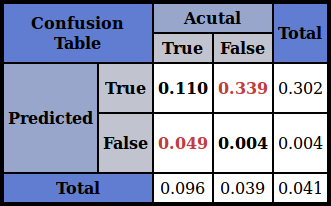
\includegraphics[width=0.3\textwidth]{Bilder/hour_min_avg_hours_changed.jpg}}
		\hfill
		\subfloat[Mittlere Anzahl an geänderten Stunden pro Regel]{\label{fig1:EMgSpR}
			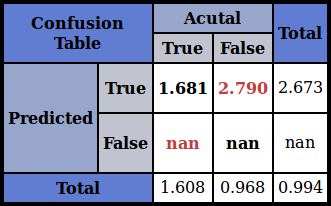
\includegraphics[width=0.3\textwidth]{Bilder/hour_min_avg_num_hours_changed.jpg}}
	\hspace*{\fill}%
	\label{fig:EMSpR}
\end{figure}
\autoref{fig:EMSpR} zeigt noch einmal, dass eine einfache Erhöhung der Mindeststundenanzahl noch keine Abhilfe schafft. Die Mindestanzahl wurde hier von 3 auf 5 erhöht. Bei den letztendlichen Klassifikationen wurde so keinerlei Verbesserungen erzeugt. Die Änderung hat lediglich bewirkt, dass noch häufiger und noch mehr Stunden lediglich aufgrund ihrer Umgebung in die Intervalle aufgenommen wurden.\\

%fazit.tex
\chapter{Fazit}
\label{sec:Fazit}

\section{Zusammenfassung}
Die Auswertung hat gezeigt, dass es prinzipiell möglich ist, vorhandene Regeln in dem Preisverhalten von Tankstellen zu erkennen. Sie hat jedoch auch gezeigt, dass der Datensatz dies nicht besonders einfach macht. Generell anwendbare Algorithmen zur Erkennung von Kausalität sind auf die Rohdaten nicht anwendbar und würden eine extensive Vorverarbeitung benötigen. Außerdem sind in Fällen, wo diese Algorithmen verwendet werden, die inhaltlichen Zusammenhänge, also die unabhängigen Faktoren, nicht bekannt, weshalb man sich auf die reine zeitliche Korrelation verlassen muss. Im Falle dieses Problems sind nicht nur die inhaltlichen Begebenheiten sehr klar definiert mit in erster Linie auch eher abhängige Faktoren, sondern es ist durch die Beschaffenheit der Pricing-Tools sogar schon klar, wie die Kausalität in Form von Regeln im Grunde aussehen kann. Da diese semantischen Informationen zur Verfügung stehen, liegt es nahe, diese in einem auf dieses Problem speziell zugeschnittenen Algorithmus zu verwenden. Eine gute Lösung für ein derart komplexes Problem zu entwerfen bedarf mehrerer Ansätze, die jeweils erneut getestet werden müssen und nimmt somit einige Zeit in Anspruch. Ein passendes Modell zu finden verläuft demnach eher nach einem evolutionären Prozessmodell.\\
Die vorliegende Arbeit übernimmt daher eher die Funktion eines ersten Prototypen. Dies ist auch ein Grund, warum noch nicht versucht wurde, die Parameter in den Ergebnissen zu optimieren. Der erster Prototyp dient hier in erster Linie der Einschätzung, ob eine automatisierte Erkennung in diesem Fall möglich ist, wie akkurat die Trefferquote sein könnte und wie aufwändig es wäre, diese zu implementieren. Die Auswertung der Ergebnisse hat hier gezeigt, dass es noch einige Parameter gibt, die eine verbesserte Klassifikation ermöglichen sollten und die verwendeten Parameter trotz erster Verbesserungen noch weiter optimiert werden müssen. Sie hat im Gegenzug aber auch gezeigt, dass es im Bereich der $\beta$-Fehler eine recht geringe Fehlerquote gibt, die statistisch wahrscheinlich nicht erkannt werden können. Im Bereich der $\alpha$-Fehler ist eine deutlich höhere Quote an Tankstellen zu vermuten, die eine zu starke Korrelation aufweisen, als dass eine kausale Einwirkung ausgeschlossen werden könnte. In gewisser Weise besteht dort auch eine kausale Abhängigkeit, die aber dann nicht direkt, sondern nur über eine dritte Tankstelle wirksam wird. Wie gravierend Fehlklassifikationen in diesem Fall sind, hängt dann stark davon ab, zu welchem Zweck die Ergebnisse eines solchen Programmes genutzt werden würden. Zudem wird im abschließenden Kapitel noch eine Möglichkeit vorgestellt, wie auch in diesen Fällen die Fehlerquote noch gesenkt werden könnte. Es soll dabei helfen, die tatsächlichen Auslöser eines Pricings von Korrelationen zu unterscheiden. Die in der Zielsetzungen formulierte Anforderung, im Pricingverhalten eindeutig erkennbare Muster zu identifizieren, ist wie in den Ergebnissen zu sehen, größtenteils erfüllt und sollte mit der Hinzunahme von den zusätzlich ermittelten signifikanten Parametern noch verbessert werden können. Inwiefern auch weniger eindeutige Muster eindeutig klassifizierbar sind, müssen dann tiefergehende Ansätze zeigen. Dazu werden im abschließenden Kapitel noch einige Möglichkeit vorgestellt, wie solche Ansätze aussehen könnten.\\
Einen stark limitierenden Faktor stellen die sehr wenigen und nicht repräsentativen Testdaten dar. Ohne bessere Testdaten ist es schwierig, die Performanz abzuschätzen und die Parameter zu optimieren. Auch hierzu wird noch eine Möglichkeiten vorgestellt, wie auch ohne Angaben von anderen Tankstellen ein gutes Trainings- und Testszenario geschaffen werden könnte.\\

\section{Ausblick}
In diesem letzten Abschnitt sollen noch ein paar weiterführende Überlegungen vorgestellt werden, die sich im Zuge dieser Arbeit ergeben haben und als Verbesserungen vorgesehen sind, aber in der für die Auswertung verwendeten Version noch nicht implementiert werden konnten.

% \titlespacing{\subsubsection}{0pt}{12pt plus 4pt minus 2pt}{-6pt plus 2pt minus 2pt}
% \subsubsection{Ausnahmen einbinden}

\subsection{Auslöser und Korrelation unterscheiden}
Ein großes Problem der aktuellen Version ist, dass eine einzelne Preisänderung mehrere potentielle Auslöser hat, wovon jeder einzelne jeweils in den Konfidenzwert für die zugehörige Tankstelle eingeht. Es kann somit vorkommen, dass in der Summe aller gefundenen Konkurrenten insgesamt mehr Auslöser zusammenkommen als tatsächlich Reaktionen bestehen. Jede Preisänderung kann natürlich in Wirklichkeit nur einen Auslöser haben. Durch diesen Umstand werden nicht nur die tatsächlichen Auslöser, sondern auch bloße Korrelationen in der Klassifikation verwendet und verursachen die vielen $\alpha$-Fehler. Um das zu verhindern, sollen die potentiellen Auslöser einer Reaktion verglichen werden, und der wahrscheinlichste soll ausgewählt werden. Es besteht natürlich die Möglichkeit, die richtigen Auslöser so auszuschließen und das Ergebnis somit zu verschlechtern. Allein die inhaltlichen Faktoren einer Preisänderung, also die geänderten Kraftstoffsorten, Höhe und der Zeitabstand reichen nicht aus, um den Auslöser eindeutig zu identfizieren. Dieser Schritt soll in einer zweiten Analyse nach der Erstellung der Regeln durchgeführt werden. Deshalb ist auch die Minimierung der $\beta$-Fehler so wichtig, da Tankstellen, die in der ersten Runde ausgeschlossen wurden, nicht wieder mitaufgenommen werden. In der zweiten Runde werden dann nur die den Regeln entsprechenden potentiellen Auslöser nochmals untersucht. Auch hier gilt es wieder, vorher möglichst keine Regeln ausgeschlossen zu haben.\\
Für die Unterscheidung von wahren Auslösern und Korrelationen soll nun ausgenutzt werden, dass ein sehr großer Anteil der Preisänderungen einer Tankstelle reaktiv sind. Selbst Initiatoren einer Preissenkung ändern ihre Preise im Grunde, um sich selbst günstiger als die Konkurrenz darzustellen, sind also auch eine Reaktion auf die Konkurrenz. Diese Initiationen sind unter Umständen nicht an einem einzelnen Konkurrenten ausgerichtet, sollten aber nur einen sehr geringer Anteil an allen Preisänderungen darstellen. Es mag einige reaktive, nicht regelbasierte Preisanpassungen geben, die schwieriger zu erkennen sein werden, aber der Hauptanteil, zumindest bei großen Markentankstellen, sollten eindeutige regelbasierte Reaktionen sein.\\
Unter den Konkurrenten wird also eine Untergruppe gesucht, die die Anzahl der Reaktionen annähernd vollkommen erklären kann. Bei Preisänderungen mit nur einem potentiellen Auslöser ist die dazugehörige Tankstelle mit ziemlicher Sicherheit in dieser Gruppe. Wenn alle potentiellen Auslöser einer Tankstelle sich mit Preisänderungen von Tankstellen überschneiden, die sich bereits in der Gruppe befinden, könnte die Tankstelle ausgeschlossen werden. Es würde nur zu Problemen kommen, wenn sich Tankstellen mit ihren Preisänderungen komplett überschneiden, weil sie zum Beispiel aufeinander reagieren. Dann wäre es wiederum möglich, die Tankstelle mit den früheren Änderungen als Konkurrent zu erachten, weil deren Preisänderungen mindestens indirekt die Auslöser der Reaktionen sind. Zudem könnte man in solchen Fällen auch überlegen, die Geolocations noch einmal auszuwerten. Liegen die beiden grob in einer Richtung, könnte man auch die näher gelegene präferiert auswählen. Es sollte mit dieser Erweiterung aber zumindest möglich sein ,weniger konsistent korrelierende Tankstellen im Umfeld als Konkurrenten auszuschließen. 

\subsection{Gegenrichtung überprüfen}
Eine Möglichkeit, Regeln noch einmal auf ihre Gültigkeit zu überprüfen wäre es, das Konkurrenzverhalten in die Gegenrichtung zu bestimmen. Konkurrenz besteht in erster Linie durch geteiltes Kundenaufkommen, sollte demnach also eigentlich auf beiden Seiten ähnlich aufgefasst werden. Es wäre allerdings nicht möglich, dass die Summe der Abstandswerte der jeweiligen Regeln negativ ist. Würde Tankstelle A, um einen Cent günstiger sein wollen als Tankstelle B, B aber wiederum höchstens den gleichen Preis dulden, dann würde der Preis innerhalb kürzester Zeit auf ein Minimum herabfallen. Bestimmte Regelkonstellationen schließen sich also gegenseitig aus.

\subsection{Generelle Muster bei Markentankstellen überprüfen}
Die großen Markentankstellen machen einen großen Teil des Marktes aus und besitzen teilweise mehr als 1000 Tankstellen in Deutschland. Bei jeder dieser Tankstellen für jeden Konkurrenten einzeln die Regeln abzuwägen wäre erhebliche Arbeit. Man könnte untersuchen, ob zu bestimmten Gruppen von anderen Tankstellen, zum Beispiel zu anderen Marken, generell gleiche oder zumindest sehr ähnliche Regeln gewählt werden, oder ob zum Beispiel nur bestimmte Gruppen überhaupt als Konkurrenten in Frage kommen.

\subsection{Marktsimulation}
Um die Ergebnisse besser testen zu können, könnte man versuchen, künstlich einen Markt zu simulieren. Es bieten sich hier zwei verschiedene Vorgehensweisen an. Man könnte einen künstlichen frei erfundenen Markt implementieren. Dieser sollte dann genau die Breite an verschiedenem Verhalten aufweisen, das auch im wirklichen Markt vermutet wird. Dazu müssten dann einige Annahmen über die tatsächlichen Verteilungen vom Verhalten im Markt getroffen werden. An diesen künstlichen Daten könnte dann getestet werden, welches Verhalten von dem Programm erkannt werden kann und wo Probleme auftreten.\\
Alternativ dazu könnte man auch versuchen, den realen Markt so gut es geht nachzubilden und darauf basierend Vorhersagen über neuerliche Preisänderungen zu treffen. Die wirklichen Preisänderungen könnten dann dazu verwendet werden, das Modell nach und nach mit zu verbessern. Dieser Ansatz kann natürlich nur funktionieren, wenn der ganze Markt generell stark regelbasiert ist und nur wenige Änderungen impulsiv oder zufällig durchgeführt werden. 
\clearpage

\pagenumbering{Roman}
\setcounter{page}{\value{ro}}
\bibliographystyle{plainnat}
\bibliography{Sources}
\clearpage

\pagenumbering{gobble}
%eidesstatt
\addchap*{Eidesstattliche Erklärung}

Ich versichere hiermit an Eides statt, dass ich die vorliegende Bachelorarbeit selbstständig und ohne unzulässige fremde Hilfe erbracht habe. Ich habe keine anderen als die angegebenen Quellen und Hilfsmittel benutzt sowie wörtliche und sinngemäße Zitate kenntlich gemacht. Die Arbeit hat in gleicher oder ähnlicher Form noch keiner Prüfungsbehörde vorgelegen. 

\vspace*{4cm}

\begin{flushleft}
\line(1,0){250}\\
Unterschrift
\end{flushleft}

\bigskip

\begin{flushleft}
\line(1,0){250}\\
Ort, Datum
\end{flushleft}
\clearpage
\addchap*{Declaration of Authorship}

I hereby certify that the work presented here is, to the best of my knowledge and belief,
original and the result of my own investigations, except as acknowledged, and has not
been submitted, either in part or whole, for a degree at this or any other university.

\vspace*{4cm}

\begin{flushleft}
\line(1,0){250}\\
signature
\end{flushleft}

\bigskip

\begin{flushleft}
\line(1,0){250}\\
city, date
\end{flushleft}
\clearpage

\end{document}